\chapter{MC for full $\HS$ under homogeneity}\label{chap:MCfullHShomo}
\begin{chapref}
The references for this chapter are~\cite{MMMPP15,ijcar16,BOZZELLI2018}.
\end{chapref}

\minitoc\mtcskip

\lettrine[lines=3]{I}{n this chapter} we prove two fundamental results. On one hand we show that MC for $\HS$ under homogeneity over finite Kripke structures is decidable.
On the other we prove a complexity lower bound for the problem, namely, its $\EXPSPACE$-hardness. In the following description of the contents of the next sections, we detail how these results are achieved.

\paragraph{Organization of the chapter.} 
\begin{itemize}
    \item In Section~\ref{sec:KrAndindAIM}, after introducing Kripke structures, we show how these system models can be mapped into abstract interval models, where each world corresponds to a trace (finite path) of the structure: this allows us to interpret $\HS$ formulas over Kripke structures, and then to define interval-based MC. Since a Kripke structure may feature loops and thus infinitely many traces, the domain of the induced abstract interval model is infinite.
    Thus, to prove decidability of MC,
    \item in Section~\ref{sec:descr} 
    we introduce BE-descriptors, that are trees built starting from the traces of a Kripke structure $\Ku$, whose nodes have labels over states of $\Ku$, which allow us to define an equivalence relation of finite index over traces of $\Ku$, parametric in the nesting depth of modalities $\hsB$ and $\hsE$ in the formula $\psi$ to check.
    \item We prove in Section~\ref{sec:decidProof} that such a relation represents a sufficient condition for two (related) traces to be indistinguishable w.r.t.\ the truth value of any $\HS$ formula with nesting depth of $\hsB$ and $\hsE$ bounded by a value equal to the depth of the considered BE-descriptors. Decidability of $\HS$ MC (under homogeneity) follows as a result of such a relation (and by minor technical ingredients). We can finally devise a \emph{nonelementary complexity} decision procedure for the problem.
    \item In Section~\ref{sec:BEhard}, we prove the $\EXPSPACE$-hardness of MC for the $\HS$ fragment $\BE$. Since MC for full $\HS$ is clearly at least as hard as MC for $\BE$, such a lower bound immediately propagates to full $\HS$. The section concludes with some remarks on the complexity gap (nonelementary--$\EXPSPACE$) deriving from the results proved for the problem.
    \item In Section~\ref{sec:overvHomo} we give an overview of the complexity of MC for several $\HS$ fragments studied under homogeneity, which will be considered in the next chapters.
    \item We conclude with Section~\ref{sec:LOMrelated}, in which we shortly review some research papers (not of the present authors) dealing with $\HS$ MC (under different semantic assumptions).
\end{itemize}

\section{Preliminaries: Kripke structures and induced abstract interval models}\label{sec:KrAndindAIM}
In the context of MC, finite state systems are usually modelled as \emph{finite Kripke structures}, 
namely, graphs where nodes represent the states of the system, edges represent transitions between states, and there is a labelling function that associates every node with a set of (atomic) properties that hold true in the corresponding system state. %Temporal logics are traditionally interpreted in terms of Kripke structures.
Systems described in terms of many modelling languages (e.g., Promela) are translated (usually, at the cost of an exponential blow-up) into Kripke structures, before the MC running phase begins. 

\begin{definition}[Kripke structure]\label{def:kripkestructure}
A Kripke structure is a tuple \[\Ku=\KuDef,\] where $\Prop$ is a finite set of proposition letters, $\States$ is a set of states (\emph{worlds}), $\Edges\subseteq \States\times \States$ is a left-total relation%
\footnote{A relation $\Edges\subseteq \States\times \States$ is left-total if, for all $s\in \States$, there exists at least one $s'\in \States$ such that $(s,s')\in\Edges$.}
between pairs of states (\emph{accessibility/transition} relation), $\Lab:\States\to 2^\mathpzc{\Prop}$ is a total labelling function, and $\sinit\in \States$ is called the \emph{initial} state.
We say that $\Ku$ is finite if $\States$ is finite.
\end{definition}
For all $s\in \States$, $\Lab(s)$ captures the set of proposition letters that hold at that state;
$\Edges$ constrains the evolution of the system over time, namely, it specifies how the system can evolve from one state to another; it is left-total because the paths of $\Ku$ are meant to represent 
system computations. 
If $(s,s')\in\Edges$, we say that $s'$ is a \emph{successor} of $s$, and $s$ a \emph{predecessor} of $s'$. By $\Edges(s)$ we denote the set of successors of $s$.

A simple Kripke structure, consisting of two states only, is reported in the following 
example. We will use it as a running example throughout the thesis.

\begin{example} \label{ex:kripke1}
Figure~\ref{K2} depicts a two-state Kripke structure 
$\Ku_2$ (the initial state is identified by a double circle).
Despite its simplicity, it features an \emph{infinite number} of different (finite) 
paths. 
%
$\Ku_2$ is defined by the 
quintuple:
\[(\{p,q\},\{s_0,s_1\},\{(s_0,s_0),(s_0,s_1),(s_1,s_0),(s_1,s_1)\},\Lab,\sinit),\]
where $\mu(s_0)=\{p\}$ and $\mu(s_1)=\{q\}$.
%$\Ku_{2}=(\mathpzc{AP},W,\delta,\mu,v_0)$ in figure \ref{K2} is an example of Kripke %structure, where:
%\begin{itemize}
%    \item $\mathpzc{AP}=\{p,q\}$;
%    \item $W=\{v_0,v_1\}$;
%    \item $\delta=\{(v_0,v_0),(v_0,v_1),(v_1,v_0),(v_1,v_1)\}$;
%    \item $\mu(v_0)=\{p\},\,\mu(v_1)=\{q\}$;
%    \item $v_0$ is the initial state (it is denoted by a double circle).
%\end{itemize}
\begin{figure}[H]
\centering
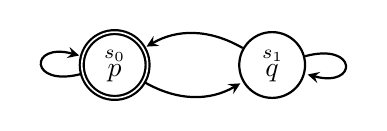
\begin{tikzpicture}[->,>=stealth,thick,shorten >=1pt,auto,node distance=2cm,every node/.style={circle,draw}]
    \node [style={double}](v0) {$\stackrel{s_0}{p}$};
    \node (v1) [right of=v0] {$\stackrel{s_1}{q}$};
    \draw (v0) to [bend right] (v1);
    \draw (v1) to [bend right] (v0);
    \draw (v0) to [loop left] (v0);
    \draw (v1) to [loop right] (v1);
\end{tikzpicture}
\caption{The finite Kripke structure $\Ku_2$.}\label{K2}
\end{figure}
\end{example}

The next definition formalizes the notion of path in a Kripke structure.
\begin{definition}[Trace over $\Ku$]
A trace $\rho$ over a Kripke structure $\Ku=\KuDef$ is a finite sequence of states $s_1\cdots s_n$, with $n\geq 1$, such that $(s_i,s_{i+1})\in \Edges$ for all $i\in\{1,\ldots ,n-1\}$.
\end{definition}

Let $\Trk_\Ku$ be the (infinite) set of all traces over a finite/infinite Kripke structure $\Ku$. For any trace $\rho=s_1\cdots s_n \in \Trk_\Ku$, we define:
\begin{itemize}
    \item $|\rho|=n$ and, for $1\leq i\leq |\rho|$, $\rho(i)=s_i$ (we also say that $i$ is a \lq\lq $\rho$-position\rq\rq );
    \item $\states(\rho)=\{s_1,\ldots,s_n\}\subseteq \States$;
    \item $\intstates(\rho)=\{s_2,\ldots,s_{n-1}\}\subseteq \States$;
    \item $\fst(\rho)=s_1$ and $\lst(\rho)=s_n$;
    \item $\rho(i,j)=s_i\cdots s_j$, for $1\leq i \leq j\leq |\rho|$, is a subtrace of $\rho$;
    \item $\Pref(\rho)=\{\rho(1,i) \mid 1\leq i\leq |\rho|-1\}$ is the set of all proper prefixes of $\rho$;
    \item $\Suff(\rho)=\{\rho(i,|\rho|) \mid 2\leq i\leq |\rho|\}$ is the set of all proper suffixes of $\rho$. 
\end{itemize}
If $\fst(\rho)=s_0$---where $s_0$ is the initial state of $\Ku$---$\rho$ is said to be an \emph{initial trace}. 

Given $\rho,\rho' \in \Trk_\mathpzc{K}$, we denote by $\rho\cdot\rho'$ the concatenation of the traces $\rho$ and $\rho'$.
Moreover, if $\lst(\rho)=\fst(\rho')$, $\rho\star \rho'$ denotes $\rho(1,|\rho|-1)\cdot \rho'$ ($\star$-concatenation). In the following, when we write $\rho\star\rho'$, we implicitly assume that
$\lst(\rho)=\fst(\rho')$.

An abstract interval model (over $\Trk_\Ku$)---recall Definition~\ref{def:AIM}---can be naturally associated with a finite Kripke structure by interpreting every trace as an interval bounded by its first and last states.
\begin{definition}[Abstract interval model induced by $\Ku$]\label{def:inducedmodel}
The abstract interval model induced by a finite Kripke structure $\Ku=\KuDef$ is the abstract interval model $\mathpzc{A}_\Ku=(\Prop,\mathbb{I},A_\mathbb{I},B_\mathbb{I},E_\mathbb{I},\sigma)$, where:
    \begin{itemize}
        \item $\mathbb{I}=\Trk_\Ku$,
        \item $A_\mathbb{I}=\left\{(\rho,\rho')\in\mathbb{I}\times\mathbb{I}\mid \lst(\rho)=\fst(\rho')\right\}$,
        \item $B_\mathbb{I}=\left\{(\rho,\rho')\in\mathbb{I}\times\mathbb{I}\mid \rho'\in\Pref(\rho)\right\}$,
        \item $E_\mathbb{I}=\left\{(\rho,\rho')\in\mathbb{I}\times\mathbb{I}\mid \rho'\in\Suff(\rho)\right\}$,
        \item $\sigma:\mathbb{I}\to 2^\Prop$ is such that, for all $\rho\in\mathbb{I}$, 
        \begin{equation*}
            \sigma(\rho)=\bigcap_{s\in\states(\rho)}\Lab(s).
        \end{equation*}
    \end{itemize}
\end{definition}
In Definition \ref{def:inducedmodel}, relations $A_\mathbb{I},B_\mathbb{I}$, and $E_\mathbb{I}$ are interpreted as Allen's interval relations $A$, $B$ and $E$, respectively. Moreover, according to the definition of $\sigma$, a proposition letter $p\in\Prop$ holds over $\rho=s_1\cdots s_n$ if and only if it holds over all the states $s_1, \ldots , s_n$ of $\rho$. This conforms to the \emph{homogeneity principle}~\cite{Roe80}, according to which a proposition letter holds over an interval if and only if it holds over all of its subintervals.

Satisfiability of an $\HS$ formula over a finite Kripke structure can now be given in terms of induced abstract interval models.
\begin{definition}[Satisfiability of $\HS$ formulas over finite Kripke structures]\label{def:satkripke}
Let $\Ku$ be a finite Kripke structure, $\rho$ be a trace in $\Trk_\Ku$,
$\psi$ be an $\HS$ formula. We say that the pair $(\Ku,\rho)$ satisfies $\psi$, denoted by $\Ku,\rho\models \psi$, if and only if it holds that $\mathpzc{A}_\Ku,\rho\models \psi$.
\end{definition}
We are now ready to formally state the \emph{MC problem} for $\HS$ over finite Kripke structures: it is the problem of deciding whether or not  $\Ku\models \psi$.
\begin{definition}[Model checking]\label{def:MCkripke}
Let $\Ku$ be a finite Kripke structure and $\psi$ be an $\HS$ formula. We say that
$\Ku$ models $\psi$, denoted by $\Ku\models \psi$, if and only if, 
for all \emph{initial} traces $\rho\in\Trk_\Ku$, it holds that $\Ku,\rho\models \psi$.
\end{definition}
It is worth pointing out that every finite Kripke structure $\Ku$ induces an abstract interval model, and that only interval models arising from finite Kripke structures are considered in the MC problem. 

Given a finite $\Ku=\KuDef$, being $\Edges$ left-total and $\States$ finite,
$\Ku$ has to feature some loops, and thus
an infinite number of traces; as a consequence, 
the \emph{MC problem is not trivially decidable}.

We conclude this section by giving some examples of meaningful properties of Kripke structures and traces that can be expressed in $\HS$. 

\begin{example}\label{example:length}
The formula $\hsBu\bot$ can be used to select all and only the traces of length $1$. Indeed, given any $\rho$ with $|\rho|=1$, independently of $\Ku$, it holds that $\Ku,\rho\models \hsBu\bot$, because $\rho$ has no proper prefixes. On the other hand, it holds that $\Ku,\rho\models \hsB\top$ if (and only if) $|\rho| > 1$.

Modality $\hsB$ can actually be used to constrain the length of an interval to be greater than, less than,  or equal to any value $k$. Let us denote $k$ nested applications of $\hsB$ by $\hsB^k$. It holds that 
$\Ku,\rho\models \hsB^k\top$ if and only if $|\rho|\geq k+1$. Analogously, $\Ku,\rho\models \hsBu^k\bot$ if and only if $|\rho|\leq k$. 
Let $\Length_k$ be a shorthand for $\hsBu^{k}\bot \wedge \hsB^{k-1}\top$. It holds that $\Ku,\rho\models \Length_k$ if and only if $|\rho|=k$ (this formula will be used several times in the next chapters).
\end{example}

\begin{example}
Let us consider again the finite Kripke structure $\Ku_2$ of Example~\ref{ex:kripke1}, depicted in Figure~\ref{K2}. For the sake of brevity, for any trace $\rho$, we denote by $\rho^n$
the trace obtained by concatenating $n$ copies of $\rho$.
%\footnote{$(v_1v_0)^3$ is a shorthand for $v_1v_0v_1v_0v_1v_0$.}
The truth of the following statements can be easily checked:
%\begin{itemize}
    ($i$)~$\Ku_2,(s_0s_1)^2\models \hsA q$;
    ($ii$)~$\Ku_2,s_0s_1s_0\not\models \hsA q$;
    ($iii$)~$\Ku_2,(s_0s_1)^2\models \hsAt p$;
    ($iv$)~$\Ku_2,s_1s_0s_1\not\models \hsAt p$.
%\end{itemize}
The above statements show that modalities $\hsA$ and $\hsAt$ can be used to distinguish between traces that \emph{start or end at different states}. 

We would like to draw attention to the \emph{branching} semantics of modalities $\hsA$ and $\hsAt$ 
(in our experience, at the beginning, this causes confusion for the reader\dots): 
$\hsA$ (resp., $\hsAt$) allows one to ``move'' to \emph{any} trace branching on the right/future (resp., left/past) of the considered one, e.g., if $\rho=s_1s_0$, then 
$\rho\, A_\mathbb{I}\, s_0$,
$\rho\, A_\mathbb{I}\, s_0s_0$, 
$\rho\, A_\mathbb{I}\, s_0s_1$, 
$\rho\, A_\mathbb{I}\, s_0s_0s_0$, 
$\rho\, A_\mathbb{I}\, s_0s_0s_1$, 
$\rho\, A_\mathbb{I}\, s_0s_1s_0s_1$, and so on.
Analogously,
$s_1\, A_\mathbb{I}\, \rho$,
$s_0s_1\, A_\mathbb{I}\, \rho$, 
$s_1s_1\, A_\mathbb{I}\, \rho$,\dots 

Figure~\ref{fig:exaAAt} illustrates the \lq\lq behaviour\rq\rq{} of $\hsA$ and $\hsAt$.

\begin{figure}[H]
    \centering
    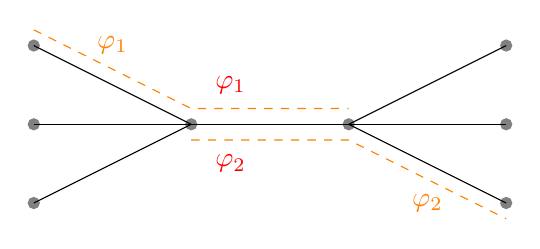
\begin{tikzpicture}
			\filldraw [gray] (4,-1) circle (2pt)
				(2,-1) circle (2pt)
				(0,0) circle (2pt)
				(0,-1) circle (2pt)
				(0,-2) circle (2pt)
				(6,0) circle (2pt)
				(6,-1) circle (2pt)
				(6,-2) circle (2pt)	;
				%
				\draw [black]  (0,-1) -- (6,-1);
				%
				\draw [black] (4,-1) -- (6,0);
				\draw [black] (4,-1) -- (6,-2);
					\draw [black] (0,0) -- (2,-1);
				\draw [black] (0,-2) -- (2,-1);
				%
				\draw [dashed, orange] (0,0.2) -> (2,-0.8) -> (4,-0.8);
				\draw [dashed, orange] (2,-1.2) -> (4,-1.2) -> (6,-2.2);
				
	%		{\tiny
				\node [orange] at (1,0) {$\varphi_1$};	
				\node [red] at (2.5,-0.5) {$\hsAt\varphi_1$};
			\node [orange] at (5,-2) {$\varphi_2$};	
				\node [red] at (2.5,-1.5) {$\hsA \varphi_2$};
		%			\node (b0) at (4,-0.5) {$\rho'=\rho(0,i)\cdot \rho^{(j+1)]}$};	
		%			\node (a1) at (1.5,0.2) {$\rho(i)=$};
		%			\node (a2) at (2,0.2) {$\rho(j)$};
		%			\node (a3) at (1.65,0.5) {$Pattern(\rho,i)= Pattern(\rho,j)$};
		%			\node (a4) at (4.6,0.5) {$Pattern(\rho,k) =\{ p \in \Prop : \Ku,\rho^{k]} \models p\}$};
						
	%			}
			\end{tikzpicture}
    \caption{The branching semantics of modalities $\hsA$ and $\hsAt$}
    \label{fig:exaAAt}
\end{figure}

Modalities $\hsB$ and $\hsE$ can be exploited to distinguish between traces encompassing a different number of iterations of a given loop. This is the case, for instance, with the following statements:
\begin{itemize}    
    \item $\Ku_2,(s_1s_0)^3 s_1\models \hsB \big(\hsA p \wedge \hsB \left(\hsA p \wedge \hsB\hsA p\right)\big)$;
    \item $\Ku_2,(s_1s_0)^2 s_1\not\models \hsB \big(\hsA p \wedge \hsB \left(\hsA p \wedge \hsB\hsA p\right)\big)$.
\end{itemize}

$\HS$ makes it possible to distinguish between traces $\rho_1=s_0^3s_1s_0$ and $\rho_2=s_0s_1s_0^3$, which involve the same number of iterations of the same loops, but differ in the order of loop occurrences: $\Ku_2,\rho_1\models \hsB\big(\hsA q \wedge \hsB(\hsA p\wedge \hsB\true)\big)$, but $\Ku_2,\rho_2\not\models \hsB\big(\hsA q \wedge \hsB(\hsA p\wedge \hsB\true)\big)$.

Also $\hsBt$ and $\hsEt$, the inverses of $\hsB$ and $\hsE$, are branching---in the future and in the past, respectively---just like $\hsA$ and $\hsAt$. See Figure~\ref{fig:exaBtEt}.

\begin{figure}[H]
    \centering
    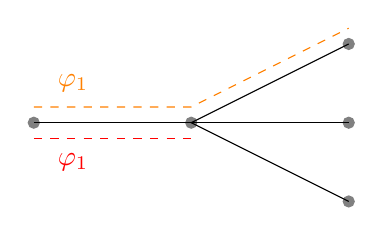
\begin{tikzpicture}
				\filldraw [gray] (0,2) circle (2pt)
				(2,2) circle (2pt)
				(4,3) circle (2pt)
				(4,2) circle (2pt)
				(4,1) circle (2pt);
				%
				
				%
				\draw [black]  (0,2) -- (4,2);
				
				%
				\draw [black] (2,2) -- (4,3);
				\draw [black] (2,2) -- (4,1);
				
				%
				\draw [dashed, orange] (0,2.2) -> (2,2.2) -> (4,3.2);
				\draw [dashed, red] (0,1.8) -> (2,1.8);
				
				
	%		{\tiny
				\node [orange] at (0.5,2.5) {$\varphi_1$};	
				\node [red] at (0.5,1.5) {$\hsBt\varphi_1$};
			
		%			\node (b0) at (4,-0.5) {$\rho'=\rho(0,i)\cdot \rho^{(j+1)]}$};	
		%			\node (a1) at (1.5,0.2) {$\rho(i)=$};
		%			\node (a2) at (2,0.2) {$\rho(j)$};
		%			\node (a3) at (1.65,0.5) {$Pattern(\rho,i)= Pattern(\rho,j)$};
		%			\node (a4) at (4.6,0.5) {$Pattern(\rho,k) =\{ p \in \Prop : \Ku,\rho^{k]} \models p\}$};
						
	%			}			
			\end{tikzpicture}
\hspace{1.1cm}
			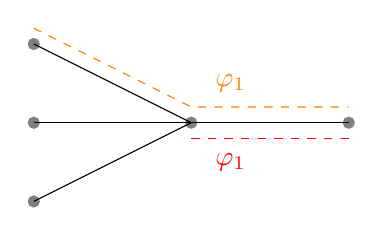
\begin{tikzpicture}
				\filldraw [gray] (4,-1) circle (2pt)
				(2,-1) circle (2pt)
				(0,0) circle (2pt)
				(0,-1) circle (2pt)
				(0,-2) circle (2pt);
				\draw [black]  (0,-1) -- (4,-1);
				\draw [black] (0,0) -- (2,-1);
				\draw [black] (0,-2) -- (2,-1);
				\draw [dashed, orange] (0,0.2) -> (2,-0.8) -> (4,-0.8);
				\draw [dashed, red] (2,-1.2) -> (4,-1.2);
				\node [orange] at (2.5,-0.5) {$\varphi_1$};	
				\node [red] at (2.5,-1.5) {$\hsEt\varphi_1$};
			\end{tikzpicture}
    \caption{The branching semantics of modalities $\hsBt$ and $\hsEt$}
    \label{fig:exaBtEt}
\end{figure}
\end{example}

\begin{example}\label{example:Ksched}
In Figure~\ref{KSched}, we give an example of a finite Kripke structure $\Ku_{Sched}$ that models the behaviour of a scheduler serving three processes which are continuously requesting the use of a common resource. 

The initial state (denoted by a double circle) 
is $s_0$: no process is served in that state. In any other state $s_i$ and $\overline{s}_i$, with $i \in \{1,2,3\}$, the $i$-th process is served (this is denoted by the fact that $p_i$ holds in those 
states). For the sake of readability, edges are marked either by $r_i$, for $\mathsf{request}(i)$, or by $u_i$, for $\mathsf{unlock}(i)$. However, edge labels do not have a semantic value, i.e., they are neither part of the structure definition, nor proposition letters; they are simply used to ease reference to edges. 

Process $i$ is served in state $s_i$, then, after ``some time'', a transition $u_i$ from $s_i$ to $\overline{s}_i$ is taken; subsequently, process $i$ cannot be served again immediately, as $s_i$ is not directly reachable from $\overline{s}_i$ (the scheduler cannot serve the same process twice in two successive rounds). A transition $r_j$, with $j\neq i$, from $\overline{s}_i$ to $s_j$ is then taken and process $j$ is served. This structure can be easily generalised to a higher number of processes.

\begin{figure}[H]
\centering
\begin{tikzpicture}[->,>=stealth',shorten >=1pt,auto,node distance=2.5cm,thick,main node/.style={circle,draw}]
  \node[main node,style={double}] (1) {$\stackrel{s_0}{\emptyset}$};
  \node[main node,fill=gray!35] (3) [below of=1] {$\stackrel{s_2}{p_2}$};
  \node[main node,fill=gray!50] (2) [left of=3] {$\stackrel{s_1}{p_1}$};
  \node[main node,fill=gray!20] (4) [right of=3] {$\stackrel{s_3}{p_3}$};
  \node[main node,fill=gray!50] (5) [below of=2] {$\stackrel{\overline{s_1}}{p_1}$};
  \node[main node,fill=gray!35] (6) [below of=3] {$\stackrel{\overline{s_2}}{p_2}$};
  \node[main node,fill=gray!20] (7) [below of=4] {$\stackrel{\overline{s_3}}{p_3}$};


  \path[every node/.style={font=\small}]
    (1) edge [bend right] node[left] {$r_1$} (2)
        edge node {$r_2$} (3)
        edge [bend left] node[right] {$r_3$} (4)
    (2) edge [bend right] node [left] {$u_1$} (5)
    (3) edge node {$u_2$} (6)
    (4) edge [bend left] node [right] {$u_3$} (7)
    (5) edge node[very near end,left] {$r_2$} (3)
    (5) edge [out=270,in=270,looseness=1.3] node [near start,swap] {$r_3$} (4)
    (6) edge node[very near end,right] {$r_1$} (2)
    (6) edge node[very near end,left] {$r_3$} (4)
    (7) edge [out=270,in=270,looseness=1.3] node [near start] {$r_1$} (2)
    (7) edge node[very near end,right] {$r_2$} (3)
    ;
\end{tikzpicture}
\vspace{-1.4cm}
\caption{The finite Kripke structure $\Ku_{Sched}$.}\label{KSched}
\end{figure}

We now show how some meaningful properties to be checked over 
%the Kripke structure 
$\Ku_{Sched}$ 
%of Figure \ref{KSched} 
can be expressed in $\HS$. 
In all formulas, we force the validity of the considered property over all legal computation sub-intervals by using modality $\hsEu$ (all computation sub-intervals are suffixes of at least one initial trace). Moreover, we will use the shorthand $wit_{\geq 2}(\{p_1,p_2,p_3\})$ for the formula
\begin{equation*}
(\hsD p_1\wedge \hsD p_2)\vee (\hsD p_1\wedge \hsD p_3)\vee (\hsD p_2\wedge \hsD p_3),
\end{equation*}
which states that there exist at least two sub-intervals such that $p_i$ holds over the former and $p_j$ over the latter, with $i,j\in\{1,2,3\}$ and $j\neq i$ (such a formula can be easily generalised to an arbitrary set of proposition letters and to any natural number $k$).

The truth of the following statements can be easily checked:
\begin{itemize}
    \item $\Ku_{Sched}\models\hsEu\left(\hsB^4\top\rightarrow wit_{\geq 2}(\{p_1,p_2,p_3\})\right)$;
    \item $\Ku_{Sched}\not\models\hsEu\left(\hsB^{10}\top\rightarrow \hsD p_3\right)$;
    \item $\Ku_{Sched}\not\models\hsEu\left(\hsB^6\top\rightarrow \hsD p_1\wedge \hsD p_2\wedge \hsD p_3\right)$.
\end{itemize}

The first formula states that in any suffix of an initial trace of length greater than or equal to 5 at least 2 proposition letters are witnessed. $\Ku_{Sched}$ satisfies the formula since a process cannot be executed twice in a row. 

The second formula states that in any suffix of an initial trace of length at least 11, process 3 is executed at least once in some internal states (\emph{non starvation}). $\Ku_{Sched}$ does not satisfy the formula since the scheduler can avoid executing a process ad libitum. 

The third formula states that in any suffix of an initial trace of length greater than or equal to 7, $p_1$, $p_2$, $p_3$ are all witnessed. The only way to satisfy this property is to constrain the scheduler to execute the three processes in a strictly periodic manner (\emph{strict alternation}), that is, $p_i p_j p_k p_i p_j p_k p_i p_j p_k\cdots$, for $i,j,k \in \{1,2,3\}$ and $i \neq  j \neq  k \neq i$, but $\Ku_{Sched}$ does not meet such a
requirement.

This example will be referred to also in the next chapters.
\end{example}


% \textbf{verificare se serve e cosa fare fino alla fine sezione}

% We show how some meaningful properties to check against 
% %the Kripke structure 
% $\Ku_{Sched}$ 
% %of Figure \ref{KSched} 
% can be expressed in HS, and, in particular, by means of formulas of the fragment $\mathsf{\overline{A}E}$---a subfragment of the fragment $\AAbarEBbarEbar$, on which we will focus in the following. 
% In all formulas, we force the validity of the considered property over all legal computation sub-intervals by using modality $[E]$ (all computation sub-intervals are suffixes of at least one initial trace). 

% Truth of the following statements can be easily checked:
% \begin{itemize}
%     \item $\Ku_{Sched}\models[E]\big(\hsE^4\top \rightarrow (\chi(p_1,p_2) \vee \chi(p_1,p_3) \vee \chi(p_2,p_3))\big)$,\\ with $\chi(p,q):=\hsE\hsAt p \wedge \hsE\hsAt q$;
%     \item $\Ku_{Sched}\not\models[E](\hsE^{10}\top \rightarrow \hsE\hsAt p_3)$;
%     \item $\Ku_{Sched}\not\models[E](\hsE^6 \rightarrow (\hsE\hsAt p_1 \wedge \hsE\hsAt p_2 \wedge \hsE\hsAt p_3))$.
% \end{itemize}
% The first formula requires that in any suffix of length at least 6 of an initial trace, at least 2 proposition letters are witnessed. $\Ku_{Sched}$ satisfies the formula since a process cannot be executed twice consecutively. 

% The second formula requires that in any suffix of length at least 12 of an initial trace, process 3 is executed at least once in some internal states. $\Ku_{Sched}$ does not satisfy the formula since the scheduler, being unfair, can avoid executing a process ad libitum. 

% The third formula requires that in any suffix of length at least 8 of an initial trace, $p_1$, $p_2$, and $p_3$ are all witnessed. The only way to satisfy this property would be to constrain the scheduler to execute the three processes in a strictly periodic manner, which is not the case.

% \textbf{verificare fin qua}

\section{The fundamental notion of $BE_k$-descriptor}\label{sec:descr}
In the previous section we have shown that, for any given finite Kripke structure $\Ku$, one can find a corresponding induced abstract interval model $\mathpzc{A}_\Ku$, featuring one interval for each trace of $\Ku$. Since $\Ku$ has loops (each state must have at least one successor, as the transition relation $\Edges$ is left-total), the number of its traces, and thus the number of intervals of $\mathpzc{A}_\Ku$, is infinite.

In this section we prove that, given a finite Kripke structure $\Ku$ and an $\HS$ formula $\varphi$, there exists a \emph{finite} representation for $\mathpzc{A}_\Ku$, equivalent to $\mathpzc{A}_\Ku$ with respect to the satisfiability of $\varphi$ (in fact, of a class of formulas including $\varphi$).

%These classes are distinguished by the notion of BE-nesting depth:
We start with the definition of some basic notions. The first one is the \mbox{BE-nesting} depth of an $\HS$ formula.

\begin{definition}[BE-nesting depth of an $\HS$ formula]\label{defnest}
Let $\psi$ be an $\HS$ formula. The BE-nesting depth of $\psi$, denoted by $\nestbe(\psi)$, is defined by induction on the structure of the formula as follows:
    \begin{itemize}
        \item $\nestbe(p)=0$ for any proposition letter $p\in\Prop$;
        \item $\nestbe(\neg\psi)=\nestbe(\psi)$;
        \item $\nestbe(\psi\wedge\varphi)=\max\{\nestbe(\psi),\nestbe(\varphi)\}$;
        \item $\nestbe(\hsB\psi)=\nestbe(\hsE\psi)=1+\nestbe(\psi)$;
        \item $\nestbe(\hsX\psi)=\nestbe(\psi)$, for $X\in\{A, \overline{A}, \overline{B},                           \overline{E}\}$.
    \end{itemize}
\end{definition}
In the following, we denote by $\nestb(\psi)$ the \lq\lq restriction\rq\rq\ of $\nestbe(\psi)$ to $\hsB$ modality only (i.e., $\nestb(\psi)$ accounts only for the nesting depth of $\hsB$ and disregards $\hsE$). Clearly $\nestb(\psi)=\nestbe(\psi)$ if $\psi$ is devoid of occurrences of $\hsE$. The analogous for $\neste(\psi)$.

Making use of the notion of BE-nesting depth of a formula, we can define a relation of $k$-equivalence over traces.
\begin{definition}[$k$-equivalence]\label{def:k-equivalence}
Let $\Ku$ be a finite Kripke structure and $\rho$ and $\rho'$ be two traces in $\Trk_\Ku$. We say that $\rho$ and $\rho'$ are $k$-equivalent if and only if, for every $\HS$ formula $\psi$ with $\nestbe(\psi)=k$, we have $\Ku,\rho\models \psi$ if and only if $\Ku,\rho'\models \psi$.
\end{definition}
It can be easily proved that $k$-equivalence \lq\lq propagates downwards\rq\rq .
\begin{proposition}
Let $\Ku$ be a finite Kripke structure and $\rho$ and $\rho'$ be two traces in $\Trk_\Ku$. If $\rho$ and $\rho'$ are $k$-equivalent, then they are $h$-equivalent, 
for all $0\leq h\leq k$.
\end{proposition}
 \begin{proof}
 Let us assume that $\Ku,\rho\models \psi$, with $0\leq \nestbe(\psi)\leq k$. Consider the formula $\hsB^k\top$, whose BE-nesting depth is equal to $k$. It trivially holds that either $\Ku,\rho\models \hsB^k\top$ or $\Ku,\rho\models \neg\hsB^k\top$. In the first case, we have that $\Ku,\rho\models \hsB^k\top \wedge \psi$. Since $\nestbe\left(\hsB^k\top \wedge \psi\right)=k$, from the hypothesis, it follows that $\Ku,\rho'\models \hsB^k\top \wedge \psi$, and thus $\Ku,\rho'\models \psi$. The other case is symmetric.
 \end{proof}

We are now ready to introduce the notion of \emph{descriptor}, which will play a fundamental role in the definition of finite abstract interval models.
%will lead to the aforementioned finite abstract model, and they are of great importance throughout the %rest of the section.

\begin{definition}[$B$-descriptor and $E$-descriptor] \label{def:descr}
Let $\Ku=\KuDef$ be a finite Kripke structure. 
A $B$-descriptor (resp., $E$-descriptor) is a labelled tree $\mathpzc{D}=(\DV,\DE,\lambda)$, where $\DV$ is a finite set of vertices, $\DE\subseteq \DV\times \DV$ is a set of edges, and $\lambda:\DV\to \States\times 2^\States\times \States$ is a node labelling function, that satisfies the following conditions:
    \begin{enumerate}
        \item for all $(v,v')\!\in\! \DE$, with $\lambda(v)\!=\!(s_{in},A,s_{fin})$ and $\lambda(v')\! =\! (s_{in}',A', s_{fin}')$, it holds that $A'\subseteq A$, $s_{in}=s_{in}'$, and $s_{fin}'\in A$
            (resp., $A'\subseteq A$, $s_{fin}=s_{fin}'$, and $s_{in}'\in A$);
        \item for all pairs of edges $(v,v'), (v,v'')\in \DE$, 
        if the subtree rooted in $v'$ is isomorphic to the subtree rooted in $v''$, then $v'=v''$
        (here and in the following, we write subtree for maximal subtree).
    \end{enumerate}
\end{definition}
(2.) of Definition \ref{def:descr} simply states that no two subtrees, whose roots are siblings, 
can be isomorphic (note that $\lambda$ is taken into account).
%\footnote{Informally, no two maximal subtrees, whose roots are siblings, can be isomorphic.}

For $X\in\{B,E\}$, the \emph{depth} of an $X$-descriptor $(\DV,\DE,\lambda)$ is the depth of the tree $(\DV,\DE)$. We call an $X$-descriptor of depth $k\in\Nat$ an $X_k$-descriptor. An $X_0$-descriptor $\mathpzc{D}$ consists of its root only, which is denoted by $\Root(\mathpzc{D})$. 
A label of a node will be referred to as a \emph{descriptor element}.
% : the notion of descriptor element bears analogies with an abstraction technique for discrete time Duration Calculus proposed by Hansen et al.\ in~\cite{HPB14}, which, on its turn, is connected to Parikh images~\cite{Par66} (a descriptor element can be seen as a qualitative analogue of this).
%
Hereafter, two descriptors will be considered \emph{equal up to isomorphism}. 

The following proposition holds.
%
\begin{proposition}\label{finitedescr}
Given a finite Kripke structure $\Ku=\KuDef$, for all $k\in\Nat$ there exists a \emph{finite number} of possible $B_k$-descriptors (resp., $E_k$-descriptors).
\end{proposition}
\begin{proof}
We consider the case of $B_k$-descriptors (the case of $E_k$-descriptors is analogous).
For $k=0$, there are at most $|S|\cdot 2^{|S|} \cdot |S|$ pairwise distinct $B_0$-descriptors. 
As for the inductive step, let us assume $h$ to be the number of pairwise distinct $B$-descriptors of depth at most $k$. The number of $B_{k+1}$-descriptors is at most $|S| \cdot 2^{|S|}\cdot |S| \cdot 2^h$ (there are at most $|S|\cdot 2^{|S|}\cdot |S|$ possible choices for the root, which can have any subset of the $h$ $B$-descriptors of depth at most $k$ as subtrees). By K\"onig's lemma, they are all finite as their depth is $k+1$ and the root has a finite number of children (no two subtrees of the root can be isomorphic).
\end{proof}

Proposition~\ref{finitedescr} provides an upper bound to the number of distinct $B_k$-descriptors (resp., $E_k$-descriptors), and thus to the number of nodes of each $B_{k+1}$-descriptor (resp., $E_{k+1}$-descriptors), for $k\in\Nat$, which is \emph{not elementary} with respect to $|S|$ and $k$, being $|S|$ the exponent and $k$ the height of the exponential tower. As a matter of fact, this is a very rough upper bound, since some descriptors may not have depth $k+1$ and some of the ``generated'' trees might not even fulfill the definition of descriptor.

We show now how $B$-descriptors and $E$-descriptors can be used to extract relevant information from the traces of a finite Kripke structure to use in MC. 
%We can now instantiate $B$-descriptors and $E$-descriptors over traces of a Kripke structure: 

Let $\Ku$ be a finite Kripke structure and $\rho$ be a trace in $\Trk_\Ku$, with $|\rho|\geq 2$.
For any $k \geq 0$, the label of the root of both the $B_k$-descriptor and $E_k$-descriptor for
$\rho$ is the triple $(\fst(\rho),\intstates(\rho),\lst(\rho))$. The root of the $B_k$-descriptor has a child for each prefix $\rho'$, with $|\rho'|\geq 2$, of $\rho$, labelled with $(\fst(\rho'),\intstates(\rho'),\lst(\rho'))$.
Such a construction is then iteratively applied to the children of the root until either depth $k$ is reached or a trace of length 2 is being considered on a node. 
The length-1 prefix of $\rho$ can be recovered as a special case, being just $\fst(\rho)$. We should associate with it a descriptor element $(\fst(\rho),\emptyset,\bot)$ as a child of the root, where $\bot$ is just a marker for \lq\lq no state\rq\rq. However, in the rest of this section, for a more uniform and elegant characterization of descriptors, we assume \emph{traces, suffixes and prefixes to have length at least 2}, as those having length 1 can always be treated as special (trivial) cases.
%
The $E_k$-descriptor is built in a similar way by considering the suffixes of $\rho$.

In general $B$- and $E$-descriptors do not convey enough information to determine which trace they were built from (this will be clear shortly). However, they can be exploited to determine which $\HS$ formulas are satisfied by the trace from which they have been built:
%\begin{itemize}
    $(i)$~to check satisfiability of proposition letters, they keep information about initial, final, and internal states of the trace;
    $(ii)$~for $\hsA\psi$ and $\hsAt\psi$ formulas, they store the final and initial states of the trace;
    $(iii)$~for $\hsB\psi$ formulas, the $B$-descriptor keeps information about all the prefixes of the trace; 
    $(iv)$~for $\hsE\psi$ formulas, the $E$-descriptor keeps information about all the suffixes of the trace;
    $(v)$~no additional information is needed for $\hsBt\psi$ and $\hsEt\psi$ formulas.
%\end{itemize}

Let $\Ku$ be a finite Kripke structure. The $B_k$-descriptor (resp., $E_k$-descriptor) for a trace $\rho$ in $\Trk_\Ku$ is formally defined as follows.
\begin{definition}[B-/E-descriptor for a trace] \label{def:tracedescr}
Let $\Ku$ be a finite Kripke structure, $\rho$ be a trace in $\Trk_\Ku$, and $k\in\Nat$. The $B_k$-descriptor (resp., $E_k$-descriptor) for $\rho$ is inductively defined as follows:
    \begin{itemize}
        \item for $k=0$, the $B_k$-descriptor (resp., $E_k$-descriptor) for $\rho$ is the tree $\mathpzc{D} = (\Root(\mathpzc{D}),\emptyset,$ $\lambda)$, where 
        \begin{equation*}
            \lambda(\Root(\mathpzc{D}))=(\fst(\rho),\intstates(\rho), \lst(\rho));
        \end{equation*}                
        
        \item for $k>0$, the $B_k$-descriptor (resp., $E_k$-descriptor) for $\rho$ is the tree $\mathpzc{D} = (\DV,\DE,\lambda)$, where 
        \begin{equation*}
            \lambda(\Root(\mathpzc{D}))=(\fst(\rho),\intstates(\rho),\lst(\rho)),
        \end{equation*}                
        which satisfies the following conditions:
%        \begin{itemize}
%            \item if $X=B$:
            \begin{enumerate}
                \item for each prefix (resp., suffix) $\rho'$ of $\rho$, there exists $v\in \DV$ such that $(\Root(\mathpzc{D}),v)\in \DE$ and the subtree rooted in $v$ is the $B_{k-1}$-descriptor (resp., $E_{k-1}$-descriptor) for $\rho'$;
                \item for each vertex $v\in \DV$ such that $(\Root(\mathpzc{D}),v)\in \DE$, there exists a prefix (resp., suffix) $\rho'$ of $\rho$ such that the subtree rooted in $v$ is the $B_{k-1}$-descriptor (resp., $E_{k-1}$-descriptor) for $\rho'$;
%            \item if $X=E$:
%            \begin{enumerate}
%                \item for each suffix $\rho'$ of $\rho$, there exists $v\in V$ such that %$(\Root(\mathpzc{D}),v)\in E$ and the maximal subtree rooted in $v$ is the $X_{k-1}$-descriptor for %$\rho'$.
%                \item for each vertex $v\in V$ such that $(\Root(\mathpzc{D}),v)\in E$, there exists a %suffix $\rho'$ of $\rho$ such that the maximal subtree rooted in $v$ is the $X_{k-1}$-descriptor for %$\rho'$.
%            \end{enumerate}
%        \end{itemize}
            \item for all pairs of edges $(\Root(\mathpzc{D}),v'), (\Root(\mathpzc{D}),v'')\in \DE$, if the subtree rooted in $v'$ is isomorphic to the subtree rooted in $v''$, then $v'=v''$.
            \end{enumerate}
    \end{itemize}
\end{definition}
%
Any $B_k$-descriptor (resp., $E_k$-descriptor) for some trace satisfies the 
conditions of Definition~\ref{def:descr} (in particular (1.)), but not vice 
versa. See the next example.

\enlargethispage{2.5\baselineskip}

\begin{example}
Consider, for instance, the $B_1$-descriptor reported in Figure~\ref{fig:wrongdesc}.
It is built on a set of states $\States$ including at least states $s_0$, $s_1$, $s_2$ and $s_3$, and it
satisfies both conditions of Definition~\ref{def:descr}. However, no trace of a finite Kripke structure can be described by it, as no trace may feature two prefixes to be associated with the first two children of the root.

\begin{figure}[H]
\centering
\begin{tikzpicture}[level distance=15mm,every node/.style={fill=gray!20}]
\Tree [.$(s_0,\{s_1,s_2\},s_3)$
    $(s_0,\{s_2\},s_1)$
    $(s_0,\{s_1\},s_2)$
    $(s_0,\emptyset,s_1)$
] 
\end{tikzpicture}
\caption{$B_1$-descriptor devoid of a corresponding trace (in any Kripke structure).}\label{fig:wrongdesc}
\end{figure}
\end{example}

\begin{example}
In Figure~\ref{Keqtr1} and \ref{Keqtr2}, we depict the $B_2$- and $E_2$-descriptors for the trace $s_0s_1s_0s_0s_1$ of the Kripke structure $\Ku_2$ of Figure~\ref{K2}.
%\ref{Keqtr1} and \ref{Keqtr2} the $B$- and $E$-descriptors of a trace of $\Ku_{2}$'s.

\begin{figure}[H]
\centering
\begin{tikzpicture}[level distance=15mm,every node/.style={fill=gray!20}]
\Tree [.$(s_0,\{s_0,s_1\},s_1)$
	[.$(s_0,\{s_0,s_1\},s_0)$
		$(s_0,\{s_1\},s_0)$
		$(s_0,\emptyset,s_1)$
]	[.$(s_0,\{s_1\},s_0)$
		$(s_0,\emptyset,s_1)$
]	$(s_0,\emptyset,s_1)$
]
\end{tikzpicture}
\caption{$B_2$-descriptor 
%$\mathpzc{D}_{B_2}$ 
for the trace  $s_0s_1s_0s_0s_1$ of $\Ku_2$.}\label{Keqtr1}
\end{figure}

\begin{figure}[H]
\centering
\begin{tikzpicture}[level distance=15mm,every node/.style={fill=gray!20}]
\Tree [.$(s_0,\{s_0,s_1\},s_1)$
	[.$(s_1,\{s_0\},s_1)$
		$(s_0,\{s_0\},s_1)$
		$(s_0,\emptyset,s_1)$
]	[.$(s_0,\{s_0\},s_1)$
		$(s_0,\emptyset,s_1)$
]	$(s_0,\emptyset,s_1)$
]
\end{tikzpicture}
\caption{$E_2$-descriptor 
%$\mathpzc{D}_{E_2}$ 
for the trace $s_0s_1s_0s_0s_1$ of $\Ku_2$.}\label{Keqtr2}
\end{figure}
\end{example}

\begin{example}
In Figure~\ref{removeisom} we show the $B_2$-descriptor for the trace $\rho = s_0s_1s_0s_0s_0s_0s_1$ of $\Ku_{2}$. It is worth noticing that there exist two distinct prefixes of the trace $\rho$, that is, the traces $\rho'=s_0s_1s_0s_0s_0s_0$ and $\rho''=s_0s_1s_0s_0s_0$, which have the same $B_1$-descriptor. Since, according to Definition~\ref{def:tracedescr}, no tree can occur more than once as a subtree of the same node (in this example, the root), in the $B_2$-descriptor for $\rho$, the prefixes $\rho'$ and $\rho''$ are represented by the same tree (the first subtree of the root on the left). This shows that, in general, the root of a descriptor for a trace with $h$ proper prefixes may have less than $h$ children.

\begin{figure}[H] 
\centering
\resizebox{\textwidth}{!}{
\begin{tikzpicture}[level distance=15mm,every node/.style={fill=gray!20}]
\Tree [.$(s_0,\{s_0,s_1\},s_1)$
	[.$(s_0,\{s_0,s_1\},s_0)$
		$(s_0,\{s_0,s_1\},s_0)$
		$(s_0,\{s_1\},s_0)$
		$(s_0,\emptyset,s_1)$
]	[.$(s_0,\{s_0,s_1\},s_0)$
		$(s_0,\{s_1\},s_0)$
		$(s_0,\emptyset,s_1)$
]	[.$(s_0,\{s_1\},s_0)$
		$(s_0,\emptyset,s_1)$
]	$(s_0,\emptyset,s_1)$
]
\end{tikzpicture}}
\caption{The $B_2$-descriptor for the trace $s_0s_1s_0s_0s_0s_0s_1$ of $\Ku_{2}$.}\label{removeisom}
\end{figure}
\end{example}

\begin{example}
This example shows that not all of the $B_k$-descriptors that can be generated from the set of states of a given finite Kripke structure are $B_k$-descriptors for some trace of that structure (the same fact is true for $E_k$-descriptors).

Let us consider the finite Kripke structure $\Ku$ in Figure~\ref{akripke} and the $B_1$-descriptor $\mathpzc{D}_{B_1}$
in Figure~\ref{akripketr}. 
By inspecting $\mathpzc{D}_{B_1}$, it can be easily checked that it can be the $B_1$-descriptor for traces of the form $s_0s_1^hs_3^2$, with $h \geq 2$, only. However, no trace of this form can be obtained by unravelling $\Ku$.

\begin{figure}[H]
\centering
\begin{tikzpicture}[->,>=stealth',shorten >=1pt,auto,node distance=1.5cm,thick,main node/.style={circle,draw}]
    \node (5) {};    
    \node[main node] (1) [above of=5] {$s_1$};
    \node[main node,style={double}] (0) [left of=5] {$s_0$};
    \node[main node] (2) [below of=5] {$s_2$};
    \node[main node] (3) [right of=5] {$s_3$};


  \path[every node/.style={font=\small}]
    (0) edge (1)
        edge (2)
    (1) edge [bend left] (2)
        edge (3)
    (2) edge [bend left] (1)
        edge (3)
    (3) edge [loop right] (3)
    ;
\end{tikzpicture}
\caption{A finite Kripke structure $\Ku$.}\label{akripke}
\end{figure}

\begin{figure}[H]
\centering
\begin{tikzpicture}[level distance=15mm,every node/.style={fill=gray!20}]
%\Tree [.$(v_0,\{v_1,v_2\},v_3)$
%        $(v_0,\{v_1\},v_2)$
%		$(v_0,\{v_2\},v_1)$
%]
\Tree [.$(s_0,\{s_1,s_3\},s_3)$
    $(s_0,\{s_1\},s_3)$
    $(s_0,\{s_1\},s_1)$
    $(s_0,\emptyset,s_1)$
] 
\end{tikzpicture}
\caption{$\mathpzc{D}_{B_1}$: a $B_1$-descriptor not corresponding to any of the traces of $\Ku$ in Figure \ref{akripke}.}\label{akripketr}
\end{figure}
\end{example}

To check an $\HS$ formula against a given finite Kripke structure we actually need to account for both the \emph{started-by} ($B$) and \emph{finished-by} ($E$) relations at the same time. To this end, we introduce $BE_k$-descriptors for traces. Given a finite Kripke structure $\Ku$ and a trace $\rho$ in $\Trk_\Ku$,
the $BE_k$-descriptor for $\rho$ can be obtained from a suitable merging of its $B_k$-descriptor and $E_k$-descriptor. It can be viewed as a sort of ``product'' of the $B_k$-descriptor and the $E_k$-descriptor for $\rho$, and it is formally defined as follows:

\begin{definition}[BE-descriptor for a trace]\label{def:BEdescr}
Let $\Ku=\KuDef$ be a finite Kripke structure, $\rho$ be a trace in $\Trk_\Ku$,
and $k \in \Nat$.
The $BE_k$-descriptor for $\rho$ is a labelled tree $\mathpzc{D}=(\DV,\DE,\lambda)$, where $\DV$ is 
a finite set of vertices, $\DE=\DE_B\cup \DE_E$, with $\DE_B\subseteq \DV\times \DV$ the set of ``$B$-edges'',
$\DE_E\subseteq \DV\times \DV$ the set of ``$E$-edges'', and $\DE_B\cap \DE_E=\emptyset$, and $\lambda:\DV\to \States\times 2^\States\times \States$, which is inductively defined on $k\in\Nat$ as follows:
    \begin{itemize}
        \item for $k=0$, the $BE_k$-descriptor for $\rho$ is $\mathpzc{D}=(\Root(\mathpzc{D}),\emptyset,\lambda)$, where 
        \begin{equation*}
            \lambda(\Root(\mathpzc{D}))=(\fst(\rho),\intstates(\rho),\lst(\rho)).
        \end{equation*}        
        
        \item for $k>0$, the $BE_k$-descriptor for $\rho$ is $\mathpzc{D}=(\DV,\DE,\lambda)$ with 
        \begin{equation*}
            \lambda(\Root(\mathpzc{D}))=(\fst(\rho),\intstates(\rho),\lst(\rho))
        \end{equation*}                
         which satisfies the following conditions:
            \begin{enumerate}
                \item[1a.] for each prefix $\rho'$ of $\rho$, there exists $v\in \DV$ such that $(\Root(\mathpzc{D}),v)\in \DE_B$ and the subtree rooted in $v$ is the $BE_{k-1}$-descriptor for $\rho'$;
                \item[1b.] for each vertex $v\in \DV$ such that $(\Root(\mathpzc{D}),v)\in \DE_B$, there exists a prefix $\rho'$ of $\rho$ such that the subtree rooted in $v$ is the $BE_{k-1}$-descriptor for $\rho'$;
                \item[1c.] for all pairs of edges $(\Root(\mathpzc{D}),v'), (\Root(\mathpzc{D}),v'') \in \DE_B$, if the subtree rooted in $v'$ is isomorphic to the  subtree rooted in $v''$, then $v'=v''$;
                \item[2a.] for each suffix $\rho''$ of $\rho$, there exists $v\in \DV$ such that $(\Root(\mathpzc{D}),v)\in \DE_E$ and the subtree rooted in $v$ is the $BE_{k-1}$-descriptor for $\rho''$;
                \item[2b.] for each vertex $v\in \DV$ such that $(\Root(\mathpzc{D}),v)\in \DE_E$, there exists a suffix $\rho''$ of $\rho$ such that the subtree rooted in $v$ is the $BE_{k-1}$-descriptor for $\rho''$;
                \item[2c.] for all pairs of edges $(\Root(\mathpzc{D}),v'), (\Root(\mathpzc{D}),v'')\in \DE_E$, if the subtree rooted in $v'$ is isomorphic to the subtree rooted in $v''$, then $v'=v''$.
            \end{enumerate}
    \end{itemize}
\end{definition}
From Definition~\ref{def:BEdescr}, it easily follows that for all $(v,v')\in \DE_B$, with $\lambda(v)=(s_{in},A,s_{fin})$ and $\lambda(v')=(s_{in}',A',s_{fin}')$, we have $A'\subseteq A$, $s_{in}=s_{in}'$, and $s_{fin}'\in A$, and  for all $(v,v')\in \DE_E$, with $\lambda(v)=(s_{in},A,s_{fin})$ and $\lambda(v')=(s_{in}',A',s_{fin}')$, we have $A'\subseteq A$, $s_{fin}=s_{fin}'$ and $s_{in}'\in A$.

%
\begin{example}
In Figure~\ref{treqdescr} at page~\pageref{treqdescr}, with reference to the finite Kripke structure $\Ku_{2}$ of Figure~\ref{K2}, we give an example of a $BE_2$-descriptor. $B$-edges are represented by solid lines, while $E$-edges are represented by dashed lines. It is worth pointing out that the $BE_2$-descriptor of Figure~\ref{treqdescr} turns out to be the $BE_2$-descriptor for both the trace $\rho=s_0s_1s_0^3s_1$ and the trace $\rho'=s_0s_1s_0^4s_1$ (and many others). As we will see very soon, this is not an exception, but the rule: different traces of a finite Kripke structure are described by the same $BE$-descriptor.
Notice also that it features two isomorphic subtrees for the same node (the root). They both consist of a single node, labelled with $(s_0,\emptyset,s_1)$. However, this does not violate Definition~\ref{def:BEdescr} since one of them is connected to the parent via a $B$-edge and the other via an $E$-edge.
\end{example}

\begin{sidewaysfigure}
\centering
\resizebox{\textheight}{!}{
\begin{tikzpicture}[level distance=30mm,every node/.style={fill=gray!20}]
\Tree [.$(s_0,\{s_0,s_1\},s_1)$
	[.$(s_0,\{s_0,s_1\},s_0)$
		$(s_0,\{s_0,s_1\},s_0)$
		$(s_0,\{s_1\},s_0)$
		$(s_0,\emptyset,s_1)$
		\edge[dashed]; $(s_1,\{s_0\},s_0)$
		\edge[dashed]; $(s_0,\{s_0\},s_0)$
		\edge[dashed]; $(s_0,\emptyset,s_0)$
]	[.$(s_0,\{s_0,s_1\},s_0)$
		$(s_0,\{s_1\},s_0)$
		$(s_0,\emptyset,s_1)$
		\edge[dashed]; $(s_1,\{s_0\},s_0)$
		\edge[dashed]; $(s_0,\emptyset,s_0)$
]	[.$(s_0,\{s_1\},s_0)$
		$(s_0,\emptyset,s_1)$
		\edge[dashed]; $(s_1,\emptyset,s_0)$
]	\textcolor{red}{$(s_0,\emptyset,s_1)$}
    \edge[dashed]; [.$(s_1,\{s_0\},s_1)$
		$(s_1,\{s_0\},s_0)$
		$(s_1,\emptyset,s_0)$
		\edge[dashed]; $(s_0,\{s_0\},s_1)$
		\edge[dashed]; $(s_0,\emptyset,s_1)$
]	\edge[dashed]; [.$(s_0,\{s_0\},s_1)$
        $(s_0,\{s_0\},s_0)$
		$(s_0,\emptyset,s_0)$
		\edge[dashed]; $(s_0,\{s_0\},s_1)$
		\edge[dashed]; $(s_0,\emptyset,s_1)$
]	\edge[dashed]; [.$(s_0,\{s_0\},s_1)$
        $(s_0,\emptyset,s_0)$
		\edge[dashed]; $(s_0,\emptyset,s_1)$
]	\edge[dashed]; \textcolor{red}{$(s_0,\emptyset,s_1)$}
]
\end{tikzpicture}}
\caption{An example of $BE_2$-descriptor.}\label{treqdescr}
\end{sidewaysfigure}

%\begin{remark}\label{remarkCutLeaves}
It can be easily checked that the $BE_{k-1}$-descriptor $\mathpzc{D}_{BE_{k-1}}$ for a trace $\rho$ can be obtained from the 
$BE_k$-descriptor $\mathpzc{D}_{BE_k}$ for $\rho$ by removing the nodes at depth $k$ (if any) and the isomorphic subtrees possibly resulting from such a removal (see (1c.) of Definition~\ref{def:BEdescr}). %In the following, we will sometimes denote $\mathpzc{D}_{BE_{k-1}}$ by $\mathpzc{D}_{BE_k}|_{k-1}$ to make it evident the way in which it is obtained.
%\end{remark}

$B_k$ and $E_k$-descriptors can be recovered from $BE_k$ ones. The $B_k$-descriptor $\mathpzc{D}_{B_k}$ for a trace $\rho$ can be obtained from the $BE_k$-descriptor $\mathpzc{D}_{BE_k}$ for $\rho$ by pruning it in such a way that only those vertices of $\mathpzc{D}_{BE_k}$ which are connected to the root via paths consisting of $B$-edges only are maintained (the set of edges of $\mathpzc{D}_{B_k}$ and its labelling function can be obtained by restricting those of $\mathpzc{D}_{BE_k}$ to the nodes of $\mathpzc{D}_{B_k}$). The $E_k$-descriptor $\mathpzc{D}_{E_k}$ of $\rho$ can be obtained in a similar way.



We focus now our attention on the relationships between the traces obtained from the unravelling of a finite Kripke structure and their $BE_k$-descriptors. A key observation is that, even though the number of traces of a finite Kripke structure $\Ku$ is infinite, for any $k\in\Nat$ the set of $BE_k$-descriptors for its traces is finite. This is an immediate consequence of Definition~\ref{def:BEdescr} and Proposition~\ref{finitedescr}. Thus, \emph{at least one $BE_k$-descriptor must be the $BE_k$-descriptor for infinitely many traces}. 

$BE_k$-descriptors naturally induce an \emph{equivalence relation of finite index} over the set of traces of a finite Kripke structure, called $k$-descriptor equivalence relation.

\begin{definition}[$k$-descriptor equivalence]
Let $\Ku$ be a finite Kripke structure, $\rho,\rho'$ be two traces in $\Trk_\Ku$,
and $k \in \Nat$. We say that $\rho$ and $\rho'$ are \emph{$k$-descriptor equivalent}, denoted by $\rho\sim_k\rho'$, if and only if the $BE_k$-descriptors for $\rho$ and $\rho'$ coincide.
\end{definition}

In the next section we will see that, for any given pair of traces $\rho,\rho'\in\Trk_\Ku$, 
%$BE_k$-descriptors and $k$-descriptor equivalence are fundamental: as  will prove, 
if $\rho\sim_k\rho'$, then $\rho$ and $\rho'$ are $k$-equivalent (see Definition \ref{def:k-equivalence}).

\section{The decidability proof}\label{sec:decidProof}

In this section we 
will see the main results behind the decidability of the MC problem for $\HS$ formulas over finite Kripke structures.
We refer to~\cite{MMMPP15} for further details and missing proofs.

As a preliminary step, we state a right extension property. Let $\Ku$ be a finite Kripke structure, $k\in\Nat$, and $\rho$ and $\rho'$ be two traces in $\Trk_\Ku$ with the same $BE_k$-descriptor (and thus, in particular, $\lst(\rho)=\lst(\rho')$). The property states that if we extend $\rho$ and $\rho'$ ``to the right'' with the same trace $\overline{\rho}$ in $\Trk_\Ku$, with $\left(\lst(\rho),\fst(\overline{\rho})\right)\in\Edges$, then the resulting traces $\rho\cdot \overline{\rho}$ and $\rho'\cdot\overline{\rho}$ (both belonging to $\Trk_\Ku$) have the same $BE_k$-descriptor as well. 
An analogous property holds for the extension of the two traces $\rho$ and $\rho'$ ``to the left'', which guarantees that $\overline{\rho}\cdot \rho$ and $\overline{\rho}\cdot \rho'$ have the same $BE_k$-descriptor (left extension property).
% In the proof, we will exploit the fact that if two traces in $\Trk_\Ku$ have the same $BE_{k+1}$-descriptor, then they also have the same $BE_k$-descriptor (see Remark \ref{remarkCutLeaves}). 

\begin{proposition}[Right extension property]\label{extLemma}
Let $\Ku=\KuDef$ be a finite Kripke structure and let $\rho$ and $\rho'$ be two traces in $\Trk_\Ku$ with $\rho\sim_k\rho'$. For any trace $\overline{\rho}$ in $\Trk_\Ku$, with $\left(\lst(\rho),\fst(\overline{\rho})\right)\in\Edges$, the two traces $\rho\cdot \overline{\rho}$ and $\rho'\cdot\overline{\rho}$ belong to $\Trk_\Ku$ and $\rho\cdot\overline{\rho}\sim_k\rho'\cdot\overline{\rho}$.
\end{proposition}

The next theorem proves that, for any pair of traces $\rho,\rho'\in\Trk_\Ku$, if $\rho\sim_k\rho'$, then $\rho$ and $\rho'$ are $k$-equivalent (see Definition \ref{def:k-equivalence}). 
\begin{theorem}\label{satPresB}
Let $\Ku$ be a finite Kripke structure, $\rho$ and $\rho'$ be two traces in $\Trk_\Ku$, and $\psi$ be a $\HS$ formula with $\nestbe(\psi)=k$. If $\rho\sim_k\rho'$ then 
$\Ku,\rho\models\psi\iff \Ku,\rho'\models\psi$.
\end{theorem}

Since the set of $BE_k$-descriptors for the traces of a finite Kripke structure $\Ku$ is finite, i.e., the equivalence relation $\sim_k$ has a finite index, there always exists a finite number of $BE_k$-descriptors that ``satisfy'' a $\HS$ formula $\psi$ with $\nestbe(\psi)= k$ (this can be formally proved by a quotient construction \cite{MMMPP15}). 

Thus we can reduce the MC problem for $\HS$ over finite Kripke structures to MC for multi-modal finite Kripke structures, whose nodes are all possible \emph{witnessed} descriptors with depth up to $k$, and there is a distinct accessibility relation for each one of the $\HS$ modalities $A$, $B$, $E$, $\overline{A}$, $\overline{B}$ and $\overline{E}$.
Since the MC problem for multi-modal finite Kripke structures is decidable (in polynomial time with respect to the size of the multi-modal Kripke structure and to the length of the formula~\cite{Gabbay87,Lan06}),
%However this does not help in the identification of a significant upper bound to the complexity 
%of our problem.} 
decidability of the MC problem for $\HS$ against finite Kripke structures follows, provided that we can effectively determine which are the descriptors witnessed (by traces) in the structure, as shown in the proof of the next theorem.
\begin{theorem} 
The MC problem for $\HS$ formulas over finite Kripke structures is decidable (with \emph{nonelementary} complexity).
\end{theorem}
\begin{proof}
Let $\Ku$ be a finite Kripke structure and let $\varphi$ be the $\HS$ formula to check, with $\nestbe(\varphi) = k$. 

We first prove that, in order to select the $BE_h$-descriptors, with $0\leq h\leq k$, witnessed by some trace in $\Ku$,
%that is, the $BE_h$-descriptors belonging to the quotient induced abstract interval model, 
we can restrict ourselves to traces devoid of prefixes associated with the same $BE_k$-descriptor.
%
Let $\rho \in \Trk_\Ku$ and let $\rho', \rho''$ be two prefixes of $\rho$, with 
$|\rho''|<|\rho'| \leq |\rho|$ (notice that we allow $\rho'$ to coincide with $\rho$).
Moreover, let $\rho = \rho' \cdot \tilde{\rho}$, for some $\tilde{\rho}$ with 
$|\tilde{\rho}| \geq 1$ (in case $|\rho| = |\rho'|$, $\rho = \rho'$).
If the $BE_k$-descriptors for $\rho'$ and $\rho''$ are the same then, by Proposition \ref{extLemma},
it holds that the $BE_k$-descriptor for $\rho'' \cdot \tilde{\rho}$ is equal to the one for 
$\rho' \cdot \tilde{\rho} = \rho$. Hence, we can safely replace $\rho$ by the $k$-descriptor equivalent 
shorter trace $\rho'' \cdot \tilde{\rho}$. 
%
We can iterate such a contraction process until there are no more pairs of prefixes associated with the same 
$BE_k$-descriptor.\footnote{As a matter of fact, the same argument can be given by referring to
suffixes instead of prefixes. Anyway, as one can easily see, making use of both the right extension 
and the left extension properties does not allow us to improve the claimed bound.}

Now, Proposition~\ref{finitedescr} provides a nonelementary upper bound to the number $\alpha$ of distinct 
$BE_h$-descriptors, with $0\leq h\leq k$ (as well as to their size), with 
respect to the size of $\Ku$ and $k$. 
%
A bound on the length of the traces in $\Trk_\Ku$ that we need to consider in order
to determine the witnessed $BE_h$-descriptors
in an effective way immediately follows: it is $1+\alpha$. 
% (it is equal to $1 + \alpha$, where $1$ must be added because the length of any trace is
% greater than or equal to $2$).

Hence, in order to generate all the witnessed $BE_h$-descriptors, with $0\leq h\leq k$, it suffices
to list, for all states $s$ of $\Ku$, all the traces starting from $s$, ordered by length,
until the above bound is reached, and then to build the corresponding $BE_h$-descriptors, with 
$0\leq h\leq k$.

We conclude that the derived MC problem for multi-modal finite Kripke 
structures has to be solved over a model whose size has a nonelementary upper bound.
\end{proof}
%%%%%%%%%%%%%%%%%%%%%%%%%%%%%%

% We proved that $k$-descriptor equivalence is a sufficient condition for $k$-equiv\-a\-lence.
% However, it is not a necessary one, and the converse does not hold in general.
% In~\cite{MMMPP15}, the authors introduce the (\lq\lq looser\rq\rq) notion of
% \emph{corresponding $BE_k$-descriptors}, which represents a necessary and sufficient condition for $k$-equivalence, thus allowing us to rephrase equivalence between traces in terms of more abstract characteristics of their descriptors.




\newcommand{\Instance}{\mathcal{I}}
\newcommand{\Beg}{\textit{beg}}
\newcommand{\End}{\textit{end}}
\newcommand{\Left}{\textit{left}}
\newcommand{\Right}{\textit{right}}
\newcommand{\Down}{\textit{down}}
\newcommand{\Up}{\textit{up}}
\newcommand{\Init}{\textit{init}}
\newcommand{\Final}{\textit{final}}


\section{\EXPSPACE-hardness of MC for $\BE$}\label{sec:BEhard}

In the previous section we have seen that MC for $\HS$ can be decided in nonelementary time. 
Obviously, this does \emph{not} imply that such problem is \emph{provably} nonelementary, meaning that no algorithm with elementary complexity may exist for it. Currently, \emph{the existence of such an algorithm is still an open issue}.

Conversely, the best complexity lower bound known to date is $\EXPSPACE$-hardness. This derives from the $\HS$ fragment $\BE$, whose modalities can express properties of both interval prefixes and suffixes
simultaneously: % , which is known to be critical as far as it concerns computational complexity.
we now prove that the MC problem for $\BE$
is $\EXPSPACE$-hard; since MC for full $\HS$ is clearly at least as hard as MC for $\BE$, such a lower bound immediately propagates to full $\HS$. 
The result is obtained by a polynomial-time reduction from a \emph{domino-tiling problem for grids with rows of single exponential length}~\cite{harel92} to MC for $\BE$. 

We start with the definition of the domino-tiling problem.
%
An instance $\Instance$ of a domino-tiling problem for grids with rows of single exponential length is a tuple $\Instance =\tupleof{C,\Delta,n,d_\Init,d_\Final}$, where $C$ is a finite set of colors, $\Delta \subseteq C^{4}$ is a set of tuples $\tupleof{c_\Down,c_\Left,c_\Up,c_\Right}$ of four colors, called \emph{domino-types}, $n>0$ is a  natural number encoded in \emph{unary},
and $d_\Init,d_\Final\in\Delta$ are two distinguished domino-types (respectively, the initial and final domino-types).
The \emph{size} of $\Instance$ is defined as $|C|+|\Delta|+n$.

\begin{figure}[b]
    \centering
    \resizebox{\linewidth}{!}{\begin{tikzpicture}[node distance=0 cm,outer sep = 0pt]

%\draw[use as bounding box] (-1,301) rectangle (16,200);

\tikzstyle{cella}=[draw, rectangle,  minimum height=0.7cm, minimum width={width("dddddd")},anchor=south west];
\tikzstyle{dcella}=[draw, rectangle, dashed, minimum height=0.7cm, minimum width={width("dddddd")},anchor=south west];
%
\node[cella] (k-0) at (0,300) {$d^k_0$};
\node[cella] (k-1) [right = of k-0] {$d^k_1$};
\node[cella] (k-2) [right = of k-1] {$d^k_2$};
\node[dcella] (k-3) [right = of k-2] {};
\node[dcella] (k-4) [right = of k-3] {};
\node[dcella] (k-5) [right = of k-4] {};
\node[cella] (k-6) [right = of k-5] {$d^k_{2^n-2}$};
\node[cella] (k-7) [right = of k-6] {$d^k_{2^n-1}$};
%
\node[dcella] (k1-4) [below = of k-4] {};
\node[cella] (k2-4) [below = of k1-4] {$d^{j+1}_i$};
\node[cella] (k3-4) [below = of k2-4] {$d^{j}_i$};
\node[cella] (k4-4) [below = of k3-4] {$d^{j-1}_i$};
\node[cella] (k3-3) [left = of k3-4] {$d^{j}_{i-1}$};
\node[cella] (k3-5) [right = of k3-4] {$d^{j}_{i+1}$};
\node[dcella] (k5-4) [below = of k4-4] {};
%
%\node[cella] (k-0)  {$d^k_0$};
\node[dcella] (1-4) [below = of k5-4] {};
\node[dcella] (1-5) [right = of 1-4] {};
\node[dcella] (1-3) [left = of 1-4] {};
\node[cella] (1-2) [left = of 1-3] {$d^0_2$};
\node[cella] (1-1) [left = of 1-2] {$d^0_1$};
\node[cella] (1-0) [left = of 1-1] {$d^0_0$};
\node[cella] (1-6) [right = of 1-5] {$d^0_{2^n-2}$};
\node[cella] (1-7) [right = of 1-6] {$d^0_{2^n-1}$};
%
 \node [align=left,red](13) [left = of 1-0] {$d_{init}$};
 \node [align=left,red](13) [right = of k-7] {$d_{final}$};
%
\node[cella] (k-k) at (10.9,298) {$d^j_i$};
\node [align=left,red] [left = of k-k] {$[d^j_i]_\Left$};
\node [align=left,red] [right = of k-k] {$[d^j_i]_\Right$};
\node [align=left,red] [below = of k-k] {$[d^j_i]_\Down =$};
\node [align=left,red] [above = of k-k] {$[d^j_i]_\Up$};
%
\node[cella] (k-k-1) at (10.9,296) {$d^{j-1}_i$};
\node [align=left,red] [above = of k-k-1] {$[d^{j-1}_i]_\Up$};
%
\node[dcella] (i-0) [below = of k-0] {};
\node[dcella] (i-1) [below = of i-0] {};
\node[dcella] (i-2) [below = of i-1] {};
\node[dcella] (i-3) [below = of i-2] {};
\node[dcella] (i-4) [below = of i-3] {};
%
\node[dcella] (j-0) [below = of k-7] {};
\node[dcella] (j-1) [below = of j-0] {};
\node[dcella] (j-2) [below = of j-1] {};
\node[dcella] (j-3) [below = of j-2] {};
\node[dcella] (j-4) [below = of j-3] {};

\end{tikzpicture}
}
%    \vspace{-0.4cm}
    \caption{A (generic) instance of the domino-tiling problem, where $d^i_j$ denotes $f(i,j)$.}\label{fig:til}
\end{figure}

Intuitively, a tiling of a grid is a color labelling of the edges of each cell (see Figure~\ref{fig:til}).
%
Formally, a \emph{tiling of $\Instance$}  is a mapping $f:[0,k]\times [0,2^{n}-1] \rightarrow \Delta$, for some $k\geq 0$, that satisfies the following constraints:
%
\begin{itemize}
  \item two adjacent cells in a row have the same color on the shared edge, namely, for all $(i,j)\in [0,k]\times [0,2^{n}-2]$,
   $[f(i,j)]_{\Right}=[f(i,j+1)]_{\Left}$ (\emph{horizontal requirement});
  \item two adjacent cells in a column have the same color on the shared edge, namely, for all $(i,j)\in [0,k-1]\times [0,2^{n}-1]$,
   $[f(i,j)]_{\Up}=[f(i+1,j)]_{\Down}$ (\emph{vertical requirement});
  \item $f(0,0)=d_\Init$ (\emph{initialization requirement}) and $f(k,2^{n}-1)=d_\Final$ (\emph{acceptance requirement}).
\end{itemize}
%

Checking the existence (respectively, non-existence) of a tiling of $\Instance$ is an $\EXPSPACE$-complete problem~\cite{harel92}.

%Since, clearly, MC for full $\HS$ is at least as hard as MC for $\BE$, the stated lower-bound immediately propagates to MC for formulas of full $\HS$.
%\begin{proof}
%
%Theorem~\ref{theorem:lowerBoundBE} is proved by a polynomial-time reduction from a domino-tiling problem for grids with rows of single exponential length~\cite{harel92}.

We now show how the domino-tiling problem can be reduced in polynomial time to the MC problem for $\BE$.
In particular, we show how to build in polynomial time a finite Kripke structure $\Ku_\Instance$ and a $\BE$ formula $\varphi_\Instance$ such that there exists an initial trace of $\Ku_\Instance$ satisfying $\varphi_\Instance$ if and only if there exists a tiling of $\Instance$. Hence, $\Ku_\Instance\models\neg\varphi_\Instance$ if and only if there is no tiling of $\Instance$.
%and  Theorem~\ref{theorem:lowerBoundBE} follows.

The encoding of tilings exploits the set of proposition letters $\Prop = \Delta \cup \{\$,0,1\}$.
%to encode tilings of $\Instance$:
%\[
%\Prop = \Delta \cup \{\$,0,1\}
%\]
%
Proposition letters in $\{0,1\}$  are used for the binary encoding of the value of an $n$-bit counter numbering the cells of a row of a  tiling, while the proposition letter $\$$ is used as a separator.
In particular, a cell with content $d\in\Delta$ and column number $j\in [0,2^{n}-1]$ is encoded by the word of length $n+1$ over $\Prop$
given by $d \,b_1\cdots b_n$,
 where $b_1 \cdots b_n$ is the binary encoding of the column number $j$ ($b_n$ being the most significant bit). A row is then represented by the word listing the encodings of cells from left to right, and a tiling $f$  consisting of  $k+1$ rows is encoded by the finite word $r_0 \$ r_1 \cdots \$ r_k$, where $r_i$ is the encoding of the
  $i$-th row of $f$, for all $i\in [0,k]$. See Figure~\ref{fig:row} for a graphical account of a word encoding of a tiling.
  
\begin{figure}[tb]
    \centering
    \resizebox{\linewidth}{!}{\newcommand{\cellTwo}[2]{
    \begin{tabular}{c|c}
        \rule[-1ex]{0pt}{3.5ex}
    #1 & #2 \\
    \end{tabular}}

\newcommand{\cellOne}[1]{
    \begin{tabular}{c}
		\rule[-1ex]{0pt}{3.5ex}
		#1
	\end{tabular}}
	
	

\begin{tikzpicture}[node distance=0 cm,->,>=stealth',shorten >=1pt,auto,semithick,main node/.style={rectangle,draw, inner sep=0pt}]  

\tikzstyle{gray node}=[fill=gray!30]
%
 \node [main node](0) at (-4,0) {\cellTwo{$d^0_0$}{$0\cdots 00$}};
 \node [main node](1) [right = of 0] {\cellTwo{$d^0_1$}{$1\cdots 00$}};
\node [main node](11) [right = of 1] {\cellOne{$\cdots$}};
 \node [main node](2) [right = of 11] {\cellTwo{$d^0_{2^n-1}$}{$1\cdots 11$}};
 \node [main node, red](3) [right = of 2]  {\cellOne{\$}};
 %
  \node [main node](4) [right = of 3]  {\cellTwo{$d^1_0$}{$0\cdots 00$}};
   \node [main node](5) [right = of 4]  {\cellTwo{$d^1_1$}{$1\cdots 00$}};
\node [main node](55) [right = of 5] {\cellOne{$\cdots$}};
   \node [main node](6) [right = of 55]  {\cellTwo{$d^1_{2^n-1}$}{$1\cdots 11$}};
   \node [main node, red](7) [right = of 6]  {\cellOne{\$}};
   \node (8) [right = of 7] {\Large $\cdots$};
   
   %
   \node [align=left,red](10) [below = of 0] {column $0$};
   \node [align=left,red](11) [below = of 1] {column $1$};
   \node [align=left,red](12) [below = of 2] {column $2^n - 1$};
   %
   \node [align=left,red](13) [below = of 4] {column $0$};
   \node [align=left,red](14) [below = of 5] {column $1$};
   \node [align=left,red](15) [below = of 6] {column $2^n - 1$};
   %
 \node [align=left,red](20) at (-4,1.2) {row $0$};
  \node [align=left,red](20) at (5.2,1.2) {row $1$};
 
\draw [{|-|},dashed,red,thick] (-5.2,1) -- (3.5,1);
\draw [{|-|},dashed,red,thick] (4.1,1) -- (12.8,1);   


%\path
%(10) edge [swap] node {} (0)
%(11) edge [swap] node {} (1)
%(12) edge [swap] node {} (2)
%(13) edge [swap] node {} (4)
%(14) edge [swap] node {} (5)
%(15) edge [swap] node {} (6);
%    \path
%    (1) edge [swap] node {hardness} (0) 
%    (0) edge  [out=150,in=190] node {hardness} (5.south)
%    (4.west) edge [swap,near end] node {hardness} (3.east)
%    (4.west) edge [near end] node {hardness} (53.east)
%    (2.north east) edge [swap,out=370,in=170] node {upper-bound} (22.north west)
%    (22.south west) edge [swap,out=190,in=-10] node {hardness} (2.south east)
%    (9) edge [swap] node {hardness} (10)
%    (21.north) edge node {hardness} (31.south)
%    (1.west) edge [swap] node {hardness} (32.south);
%    
%    \draw [dashed,-,red,thick] (-6.5,4) -- (6,4);
%    \draw [dashed,-,gray] (-6.5,-2.5) -- (6,-2.5);
%    \draw [dashed,-,gray] (-6.5,-0.5) -- (6,-0.5);
%    
%    \node[align=left](50) at (4,-5) {
%    $^1$ \cite{MMMPP15}, 
%    $^2$ \cite{MMP15}, 
%    $^3$ \cite{MMP15B}, 
%    $^4$ \cite{MMPS16}};

\end{tikzpicture}}
    \vspace{-0.4cm}
    \caption{Encoding of a tiling as a word, where $d^i_j$ denotes $f(i,j)$.}\label{fig:row}
\end{figure}

%\paragraph{Construction of $\Ku_\Instance$ and $\varphi_\Instance$}
The Kripke structure $\Ku_\Instance$ is trivially defined as
 \[
 \Ku_\Instance = \tpl{\Prop, \Prop, \Prop\times \Prop, \Lab,d_\Init}
 ,\]
 where $\Lab(p)=\{p\}$, for each $p\in\Prop$. Thus, the initial traces of $\Ku_\Instance$ correspond to the finite words over $\Prop$ which start with the initial domino type $d_\Init$.
 
In order to build the $\BE$ formula $\varphi_\Instance$, we use some auxiliary formulas, namely, $\Length_i$, $\Beg(p)$, $\End(p)$, $\phi_{\textit{cell}}$, and $\theta_j(b,b')$, where $i\in [1,2n+2]$, $j\in [2,n+1]$, $p\in \Prop$, and $b,b'\in \{0,1\}$.

The formula  $\Length_i$, already presented in Example~\ref{example:length}, has size linear in $i$ and characterizes the traces having length $i$: %It can be expressed as follows:
\[
\Length_i= \hsBu^{i} \bot \wedge \hsB^{i-1} \top.
\]
The formula $\Beg(p)$ (resp., $\End(p)$) captures the traces of $\Ku$ which start (resp., end) in the state $p$:
\[
\Beg(p)= (p\wedge \Length_1) \vee \hsB(p\wedge \Length_1),
\quad
\End(p)= (p\wedge \Length_1) \vee \hsE(p\wedge \Length_1).
\]
The formula $\phi_{\textit{cell}}$ captures the traces of $\Ku_\Instance$ which encode cells:
\[
\phi_{\textit{cell}}= \Length_{n+1}\wedge \Big(\displaystyle{\bigvee_{d\in \Delta} \Beg(d)}\Big)\wedge \hsEu(\Beg(0)\vee \Beg(1)).
\]
%
Finally, for all $j\in [2,n+1]$ and $b,b'\in \{0,1\}$, the formula $\theta_j(b,b')$ is defined as:
\[
\theta_j(b,b')= \hsB(\Length_j \wedge \End(b))\wedge \hsE(\Length_{n-j+2} \wedge \Beg(b')).
\]
It is satisfied by a trace $\rho$ if $|\rho|\geq j+1$, $|\rho|\geq n-j+3$, $\rho(j)= b$, and $\rho(|\rho|-n+j-1)=b'$. In particular, for a trace $\rho$ starting with a cell $c$ and ending with a cell $c'$, $\theta_j(b,b')$ is satisfied by $\rho$ if the $(j-1)$-th bit of $c$ is $b$ and the $(j-1)$-th bit of $c'$ is $b'$. See Figure \ref{fig:thetaj} for an example.
\begin{figure}[t]
    \centering
    \scalebox{0.4}{\includegraphics{Chaps/Intro/thetaj.pdf}}
    \caption{Encoding of a trace $\rho$ starting with a cell $c=(d\, 1001)$ and ending with a cell $c'=(d'\, 1101)$ (here, $n=4$). The formula $\theta_2(1,1)$ is satisfied by $\rho$, while $\theta_3(1,0)$ is not.}
    \label{fig:thetaj}
\end{figure}

Additionally, we use the derived operator $\hsG$ and its dual $\hsGu$, which allow us to select  arbitrary subtraces of the given trace, including the trace itself:
\[
\hsG\psi= \psi \vee \hsB\psi \vee \hsE\psi \vee \hsB\hsE\psi.
\]

The formula $\varphi_\Instance$ is defined as follows:
\[
\varphi_\Instance= \varphi_{\textit{b}} \wedge \varphi_{\textit{req}}\wedge \varphi_{\textit{inc}}\wedge \varphi_{\textit{rr}}\wedge \varphi_{\textit{rc}}.
\]
The conjunct $\varphi_{\textit{b}}$ checks that the given trace starts with a cell with content $d_\Init$ and column number $0$, and ends with a cell with content $d_\Final$
and column number $2^{n}-1$:
\[
\varphi_{\textit{b}} = \hsB\phi_{\textit{cell}}\wedge \Beg(d_\Init) \wedge  \hsE(\phi_{\textit{cell}} \wedge \Beg(d_\Final)) \wedge
\displaystyle{\bigwedge_{j=2}^{n+1}}\theta_j(0,1). 
\]
%
The conjunct $\varphi_{\textit{req}}$ ensures the following two requirements:
$(i)$ each occurrence of $\$$ in the given trace is followed by a cell with column number $0$ and
$(ii)$ each cell $c$ in the given trace is followed either by another cell, or by the separator $\$$, and in the latter case $c$ has column number $2^{n}-1$.
%
The first requirement is encoded by the formula: % follows:
\[
\hsGu\bigl((\Length_{n+2} \wedge \Beg(\$)) \longrightarrow \hsE(\phi_{\textit{cell}}\wedge \hsEu\Beg(0))\bigr);
\]
the second one by the formula:
\begin{multline*}
\hsGu\Bigl\{(\Length_{n+2} \wedge \displaystyle{\bigvee_{d\in \Delta}} \Beg(d)) \longrightarrow\\
\Bigl(\hsB\phi_{\textit{cell}} \,\wedge\,  (\End(\$)\vee \displaystyle{\bigvee_{d\in \Delta}} \End(d))\, \wedge\, (\End(\$) \longrightarrow \hsEu(\Beg(\$)\vee \Beg(1)))\Bigr)\Bigr\}.
\end{multline*}
%
The conjunct $\varphi_{\textit{inc}}$  checks that adjacent cells along the given trace have consecutive columns numbers:
%
\[
\varphi_{\textit{inc}} = \hsGu\Bigl( \phi_{\textit{two\_cells}} \longrightarrow \displaystyle{\bigvee_{j=2}^{n+1}}\bigl[\theta_j(0,1)\wedge \bigwedge_{h=2}^{j-1}\theta_h(1,0) \wedge \bigwedge_{h=j+1}^{n+1}\bigvee_{b\in\{0,1\}}\theta_h(b,b)\bigr]\Bigr ),
\]
where $\phi_{\textit{two\_cells}}$ is given by
$
\Length_{2n+2}\wedge  \hsB\phi_{\textit{cell}}\wedge  \hsE\phi_{\textit{cell}}
$.
%
Note that $\varphi_{\textit{req}}$ and $\varphi_{\textit{inc}}$ ensure that column numbers are correctly encoded.

The conjunct $\varphi_{\textit{rr}}$  checks that adjacent cells in a row   have the same color on the shared edge:
\[
\varphi_{\textit{rr}} = \hsGu\Bigl( \phi_{\textit{two\_cells}} \longrightarrow\quad \smashoperator{\bigvee_{(d,d')\in \Delta\times \Delta\mid d_{\Right}= d'_{\Left}}} \quad (\Beg(d) \wedge \hsE(\Length_{n+1}\wedge \Beg(d')))\Bigr ) .
\]
%
Finally, the conjunct   $\varphi_{\textit{rc}}$  checks that adjacent cells in a column  have the same color on the shared edge.
For this, it suffices to require that
the following condition holds:
\begin{itemize}
  \item for each subtrace of the given one containing exactly one occurrence of $\$$, starting with a cell $c$, and ending with a cell $c'$, if $c$ and $c'$ have the same column number, then $d_{\Up}= d'_{\Down}$, where $d$ (respectively, $d'$) is the content of $c$ (respectively, $c'$).
\end{itemize}
%
Accordingly, the formula $\varphi_{\textit{rc}}$ is defined as follows, where we use the formulas $\theta_j(b,b)$, with $j\in [2,n+1]$ and $b\in \{0,1\}$, to express that $c$ and $c'$ have the same column number:
\begin{multline*}
  \varphi_{\textit{rc}} = \hsGu\Bigl\{\,\, \Big(\phi_{\textit{one}}(\$) \,\,\wedge \,\, \hsB\phi_{\textit{cell}} \,\,\wedge \,\, \hsE\phi_{\textit{cell}} \,\,\wedge \,\, \displaystyle{\bigwedge_{j=2}^{n+1}\bigvee_{b\in \{0,1\}}}\theta_j(b,b)\,\,\Bigr)\\
  \longrightarrow \smashoperator[r]{\bigvee_{(d,d')\in \Delta\times \Delta\mid d_{\Up}= d'_{\Down}}}\quad (\Beg(d) \wedge \hsE(\Length_{n+1}\wedge \Beg(d')))\,\,\,\Bigr\},
\end{multline*}
%
where $\phi_{\textit{one}}(\$)$ is defined as
\[
(\hsB\End(\$))\,\,\wedge\,\, \neg(\hsB(\End(\$) \wedge \hsB\End(\$)))
.\]

The formula $\varphi_\Instance$ has length polynomial in the size of $\Instance$. 
%
By construction, a trace $\rho$ of $\Ku_\Instance$ satisfies $\varphi_\Instance$ if and only if $\rho$ encodes a tiling.
Since the initial traces of $\Ku_\Instance$ are the finite words over $\Prop$ starting with $d_\Init$, it follows that there exists a tiling of $\Instance$ if and only if there exists an initial trace
of $\Ku_\Instance$ which satisfies $\varphi_\Instance$. 

The given reduction proves the following theorem. %, concluding the section.
%of Theorem~\ref{theorem:lowerBoundBE} is finished.

\begin{theorem}\label{theorem:lowerBoundBE} The MC problem for $\BE$ formulas over finite Kripke structures is \EXPSPACE-hard (under polynomial-time reductions).
\end{theorem}
%\end{proof}


Before concluding the section,
we would like to comment on the complexity gap deriving from the upper and lower bounds proved for $\HS$ (and $\BE$) MC.

Let us start by introducing \emph{star-free regular expressions} over a finite alphabet $\Sigma$, with $|\Sigma|\geq 2$, that are defined by the grammar
\[r::= \emptyset \mid a \mid r \cdot r \mid r \cup r \mid \neg r ,\]
where $a\in\Sigma$.
Every regular expression defines a language $\Lang(r)$ of finite words over $\Sigma$ by induction on its structural complexity
as follows:
%\begin{itemize}
   $\Lang(\emptyset)=\emptyset$,
   $\Lang(a)=\{a\}$,
   $\Lang(r_1\cdot r_2)=\Lang(r_1)\cdot \Lang(r_2)$,
   $\Lang(r_1\cup r_2)=\Lang(r_1)\cup \Lang(r_2)$ and
   $\Lang(\neg r)=\Sigma^*\setminus\Lang(r)$.\footnote{%
   As a standard notation, the dot $\cdot$ represents the concatenation of words, and $\Sigma^*$ (resp., $\Sigma^+$) the set of all possible \emph{finite} (resp., finite and non-empty) words over $\Sigma$.
   } 
%\end{itemize}
It is well-known that the \emph{language-emptiness problem for star-free regular expressions is (provably) nonelementary}~\cite{Stockmeyer:1973,stockmeyer1974} (more properly, \TOWER-complete in the notation of~\cite{Schmitz:2016}), being negation the \lq\lq difficult case\rq\rq.

Let us now slightly modify the definition of these expressions. We consider:
\[r::= \emptyset \mid a \mid r \cdot \Sigma^+ \mid \Sigma^+\cdot r \mid r \cup r \mid \neg r .\]
Again, negation is present and there is no Kleene star (as $\Sigma^+$ can be \lq\lq rewritten\rq\rq{} as $\neg\emptyset$); \emph{concatenation is now weakened}: in fact, $r \cdot \Sigma^+$ and $\Sigma^+\cdot r$ represent right-/left-extensions of a word in $\Lang(r)$ with any (non-empty) word.
To the best of our knowledge, nothing is known about the precise complexity of this variant of star-free regular expressions.

The reader may now be wondering why we care so much about these regular expressions. The answer is given by the following fact:
\emph{there is a trivial reduction from language emptiness for this variant of expressions to $\BE$ MC, and vice versa}.
Intuitively, $r \cdot \Sigma^+$ (resp., $\Sigma^+\cdot r$) can be \lq\lq simulated\rq\rq{} by $\hsB$ (resp., $\hsE$).%
\footnote{It is also worth noting that the \lq\lq general\rq\rq{} concatenation $r\cdot r$ cannot be simulated by $\BE$: the \emph{chop} operator would be needed, which bisects an interval into two consecutive parts/subintervals: $\psi_1\langle C\rangle \psi_2$ predicates $\psi_1$ over the first subinterval and $\psi_2$ over the second.}
%
As an immediate consequence, an improvement on the known (upper or lower) bounds for any of the two problems would immediately propagate to the other.

Unfortunately, the nonelementary lower bound proved for (standard) star-free regular expressions by Stockmeyer in his PhD thesis \cite{stockmeyer1974} cannot be adapted to the variant, failing to encode the so-called \lq\lq \emph{movable rulers}\rq\rq, 
namely, regular expressions that are \lq\lq satisfied\rq\rq{} only by (all) words of a precise length.
Conversely, it is not clear how the (nonelementary) complexity of the standard automata-based algorithm for deciding the emptiness of regular expressions could possibly be lowered by exploiting the weakened concatenation; analogously, the nonelementary algorithm for full $\HS$ MC represents, at the moment, the best algorithm also for $\BE$ MC. 


\section{An overview on MC for $\HS$ and its fragments under homogeneity}
\label{sec:overvHomo}

%In the previous sections we have established two fundamental results.
%On one hand, 
%we have given a nonelementary decision procedure for solving $\HS$ MC.
%On the other, we have shown that 
As the $\EXPSPACE$-hardness of the fragment $\BE$ clearly propagates to full $\HS$, $\HS$ MC represents a \emph{provably intractable problem} (here and in the following, we say \lq\lq intractable\rq\rq---by borrowing the terminology from Meyer and Stockmeyer~\cite{Stockmeyer:1973}---when a problem can not be provably solved in polynomial time).
%
The reasons which originated a systematic, in-depth investigation on complexity and expressiveness of $\HS$ fragments should then appear obvious: lowering the computational complexity of MC has crucial importance; at the same time, identifying a good \emph{trade-off between complexity and expressiveness} of a logic is fundamental as well. In the next chapters we start considering the issue of complexity which, for $\HS$ fragments where properties of prefixes (namely, $\hsB$) and suffixes ($\hsE$) of intervals are dealt with separately, is markedly lower than that of full $\HS$ (see Figure~\ref{fGr} for a graphical overview). Expressiveness will be addressed in Chapter~\ref{chap:TOCL17}: there we will make
a comparison of different semantic variants of $\HS$; %that is, \emph{state-based} (the one adopted here), \emph{trace-based}, and \emph{computation-tree-based}, 
in addition we will compare such variants with the standard point-based temporal logics $\LTL$, $\CTL$, and $\CTLStar$.

\begin{figure}[p]
\centering
    \newcommand{\cellThree}[3]{
\begin{tabular}{c|c}
\rule[-1ex]{0pt}{3.5ex}
\multirow{2}{*}{#1} & #2 \\ 
\hhline{~=}\rule[-1ex]{0pt}{3.5ex}
 & #3 
\end{tabular}}

\newcommand{\cellTwo}[2]{\begin{tabular}{c|c}
\rule[-1ex]{0pt}{3.5ex}
#1 & #2 \\
\end{tabular}}

\newcommand{\cellOne}[1]{\begin{tabular}{c}
		\rule[-1ex]{0pt}{3.5ex}
		#1
	\end{tabular}}
	
	
\resizebox{\linewidth}{!}{
\begin{tikzpicture}[->,>=stealth',shorten >=1pt,auto,semithick,main node/.style={rectangle,draw, inner sep=0pt}]  

\tikzstyle{gray node}=[fill=gray!30]

    \node [main node](0) at (-4,0) {\cellTwo{$\AAbarBbarEbar$}{$\Psp$-complete}};
    \node [main node](1) at (3,0)  {\cellTwo{$\Bbar$}{$\Psp$-complete}};
    \node [main node](21) at (3,0.8)  {\cellTwo{$\Ebar$}{$\Psp$-complete}};
    \node [main node](31) at (3,2.3)  {\cellTwo{$\AAbarEEbar$}{$\Psp$-complete}};
    \node [main node](31a) at (3,3.2)  {\cellTwo{$\D$}{$\Psp$-complete}};
    \node [main node](32) at (-2.3,2.3)  {\cellTwo{$\AAbarBBbar$}{$\Psp$-complete}};
    \node [main node](2) at (-5.0,-3.4) {\cellThree{$\AAbar$}{$\Thsq$}{$\Th$-hard }};
    \node [main node](22) at (0.2,-3.4) {\cellThree{\hspace*{-6pt}$\begin{array}{c}\A, \\ \Abar \end{array}$\hspace*{-6pt}}{$\Thsq$}{$\Th$-hard }};
    \node [main node](92) at (4.8,-3.4) {\cellThree{\hspace*{-6pt}$\begin{array}{c}\Abar\B, \\ \A\E \end{array}$\hspace*{-6pt}}{$\Thsq$}{$\Th$-hard}};
    
    \node [main node](72) at (-3.3,-1.0)  {\cellTwo{$\AAbarB$}{$\PTIME^{\NP}$-complete}};
    \node [main node](73) at (3.5,-1.0)  {\cellTwo{$\AAbarE$}{$\PTIME^{\NP}$-complete}};
    \node [main node](74) at (-3.3,-2)  {\cellTwo{$\A\B$}{$\PTIME^{\NP}$-complete}};
    \node [main node](75) at (3.5,-2)  {\cellTwo{$\Abar\E$}{$\PTIME^{\NP}$-complete}};
    
    \node [main node](53) at (-4,-6) {\cellTwo{$\B$}{$\co\NP$-complete}};
    \node [main node](3) at (-4,-5) {\cellTwo{$\E$}{$\co\NP$-complete}};
    \node [main node](4) at (3.5,-5.5) {\cellTwo{$\HSprop$}{$\co\NP$-complete }};
    
    \node [main node](5) at (-4,4) {\cellThree{$\AAbarBBbarEbar$}{$\EXPSPACE$ }{$\Psp$-hard }};
    %\node [main node](6) at (-3.5,6) {\cellThree{succinct $\AAbarBBbarEbar$}{$\EXPSPACE$ }{$\NEXPTIME$-hard }};
    
    \node [main node](9) at (3,6) {\cellThree{$\BE$}{\textbf{nonELEMENTARY}}{$\EXPSPACE$-hard }};
    \node [main node](10) at (3,8) {\cellThree{full $\HS$}{\textbf{nonELEMENTARY}}{$\EXPSPACE$-hard}};
   
    \path
    (1) edge [swap] node {hard} (0) 
    (0) edge  [out=150,in=190] node {hard} (5.south)
    (4.west) edge [swap,near end] node {hard} (3.east)
    (4.west) edge [near end] node {hard} (53.east)
    (2.north east) edge [swap,out=370,in=170] node {upper-b.} (22.north west)
    (22.south west) edge [swap,out=190,in=-10] node {hard} (2.south east)
    (22.east) edge node {hard} (92.west)
    (9) edge [swap] node {hard} (10)
    (21.north) edge node {hard} (31.south)
    (1.west) edge [out=120,in=-45, near end] node {hard} (32.south)
    (74.west) edge [out=130, in=230, near end] node {hard} (72.west)
    (72.east) edge [out=310, in=50] node {upper-bound} (74.east)
    (75.west) edge [out=130, in=230, near end] node {hard} (73.west)
    (73.east) edge [out=310, in=50] node {upper-b.} (75.east)
    ;
    
    \draw [dashed,-,red] (-6.5,4) -- (6,4);
    \draw [dashed,-,red] (-6.5,-2.5) -- (6,-2.5);
    \draw [dashed,-,red] (-6.5,-4.5) -- (6,-4.5);
    \draw [dashed,-,red] (-6.5,-0.5) -- (6,-0.5);
    
    
    \draw [->,blue] (0,8) .. controls (0.1,3) .. node [right] {Chap.~\ref{chap:ICALP}} (0.8,3.3) ;
    \draw [->,blue] (0.5,2.2) .. controls (-0.4,3.5) and (-1.3,2.3) .. node [right, very near end] {Chap.~\ref{chap:TCS17}} (-1.8,3.4);
    \draw [->,blue] (0.5,2) .. controls (0.1,-0.8) .. node [left, near end] {Chap.~\ref{chap:IC17}} (-0.5,-1.4);
    \draw [->,blue] (0,-0.8) .. controls (0.7,-1.2) .. (1.2,-2.8);
\end{tikzpicture}
}
    %\vspace{-0.4cm}
    \caption{Complexity of the MC problem for $\HS$ and its fragments. Red lines separate different complexity classes. Blue arrows depict the contents of the next three chapters.}
    \label{fGr}
\end{figure}

Since the combined use of modalities for prefixes $\hsB$ and suffixes $\hsE$ is critical,
the first fragments taken into consideration were 
$\AAbarBBbarEbar$ and $\AAbarEBbarEbar$:
these (syntactically maximal) fragments are obtained from full $\HS$ (i.e., $\AAbar\BE\Bbar\Ebar$) in an obvious way, that is, by removing either $\B$ or $\E$.
In~\cite{MMP15} we devised, for both of them, an $\EXPSPACE$ MC algorithm which finds, for each trace of the input Kripke structure, a satisfaction-preserving trace of bounded exponential length, i.e., a \emph{trace representative}. In this way, the algorithm needs to check only trace representatives instead of traces of unbounded length. In the same paper, it was proved that formulas satisfying a constant bound on the B-nesting depth (resp., E-nesting depth) can be checked in polynomial working space. As a consequence MC for $\AAbar\Bbar\Ebar$ is in $\PSPACE$ (its formulas do not feature $\hsB$/$\hsE$, hence $\nestb(\psi)=\neste(\psi)=0$).
The techniques employed in~\cite{MMP15} will be summarized at the beginning of Section~\ref{sec:AAbarBBbarEbar}.
However, the proof of existence of trace representatives is rather involved and it exploits very technical arguments. In this thesis, we will prove---in a (hopefully!) much more understandable and compact way---membership to $\EXPSPACE$ of MC for $\AAbarBBbarEbar$ and $\AAbarEBbarEbar$ (Section~\ref{sec:AAbarBBbarEbar}) by having recourse to completely different notions.

Still in Chapter~\ref{chap:TCS17} (Section~\ref{sec:AAbarEEbar}), we prove that MC for the $\HS$ fragment $\AAbarBBbar$ (resp., $\AAbarEEbar$) %that allows one to express properties of future and past intervals, interval prefixes (resp., suffixes), and right (resp., left) interval extensions, 
is in $\PSPACE$.
Since MC for the $\HS$ fragment featuring only one modality for right (resp., left) interval extensions $\Bbar$ (resp., $\Ebar$) is $\PSPACE$-hard (see Appendix~\ref{sect:BbarHard}),%
\footnote{The $\PSPACE$-hardness of MC for $\Bbar$/$\Ebar$ gives the best (unmatching) complexity lower bound also for $\AAbarBBbarEbar$ and $\AAbarEBbarEbar$ MC.}
$\PSPACE$-completeness immediately follows: 
the complexity turns out be the same as the one of $\LTL$ MC (known to be $\PSPACE$-complete~\cite{Sistla:1985}).
As a \lq\lq byproduct\rq\rq , we show that MC for the one-modality fragments $\B$ and $\E$ ($\B$ and $\E$ dealt with separately!) turns out to be $\co\NP$-complete.%
\footnote{The $\co\NP$-hardness derives from that of the fragment $\HSprop$ (the purely propositional fragment of $\HS$), as proved in~\cite{MMP15B}.}
These results are achieved by means of a \emph{small-model property}: intuitively, given a trace $\rho$ in a finite Kripke structure and a formula $\varphi$ of $\AAbarBBbar$/$\AAbarEEbar$, we prove that, by iteratively contracting $\rho$ it is always possible to build another trace
whose length is \emph{polynomially bounded} in the size of the formula and of the Kripke structure, which preserves the satisfiability of  $\varphi$  with respect to  $\rho$. 

In Chapter~\ref{chap:IC17}, we analyze the sub-fragments of $\AAbarBBbar$ (respectively, $\AAbarEEbar$), which are still expressive enough to capture meaningful interval properties of state transition systems and whose MC problem has a computational complexity markedly lower than that of full $\HS$,
namely, $\A$, $\Abar$, $\AAbar$, $\AB$, $\AbarB$, $\AE$, $\AbarE$, $\AAbarB$, and  $\AAbarE$.
%What they have in common is the 
All these have a similar computational complexity, as their MC problem settles in one of the lowest levels of the \emph{polynomial-time hierarchy}, $\PTIME^{\NP}$, or below. Such a class consists of the set of problems decided by a deterministic polynomial-time bounded Turing machine, with the \lq\lq support\rq\rq{} of an oracle for the class $\NP$,
that is, a tool which decides, in one computation step, whether an instance of a problem belonging to $\NP$ is positive or not. 
%As a consequence, similar techniques can be applied to provide asymptotically optimal model checking algorithms, and analogous ideas can be exploited to prove their hardness.
$\PTIME^{\NP}$ is also referred to as $\PTIME$ \emph{relative to} $\NP$ (relativization).
%
However, though the fragments in the considered set are similar, some differences can be marked. In particular, the fragments $\A$, $\Abar$, $\AAbar$, $\AbarB$, and $\AE$ are actually \lq\lq easier\rq\rq{} than the other ones, since they require the $\PTIME$ Turing machine to perform just $O(\log^2 n)$ queries to the $\NP$ oracle, for an input size $n$, instead of $O(n^k)$ queries, for some constant $k\geq 0$, as it is allowed in the general case for a  polynomial running time machine. The MC problem for these fragments witnesses
%\lq\lq generates\rq\rq 
a \lq\lq non-standard\rq\rq{} complexity class in the polynomial-time hierarchy, called \emph{bounded-query} class, that will be presented in detail in Section~\ref{sub:compl}.
%
More precisely, 
we devise a $\PTIME^{\NP}$ MC algorithm for $\AAbarB$ and $\AAbarE$ in Section~\ref{sec:AAbarBalgo}, and then prove a matching complexity lower bound (Section~\ref{sec:ABhard});
then we show that MC for $\A$, $\Abar$, $\AAbar$, $\AbarB$ and $\AE$   
is still in $\PTIME^{\NP}$, but only $O(\log^2 n)$ queries to the $\NP$ oracle are necessary (Section~\ref{sect:AAbarAlg}).
This result is achieved by a reduction \emph{to} the problem TB(SAT)~\cite{schnoebelen2003}, whose instances are complex 
circuits where some of the gates are endowed with $\NP$ oracles. 
Finally, we identify a lower bound, which shows that \emph{at least $\log n$ queries} are needed to solve the problem (Section~\ref{sect:AHard}). Unfortunately, such bound does not exactly match the upper bound, leaving open the question whether the problem can be solved by $o(\log^2 n)$ (i.e., strictly less than $O(\log^2 n)$) queries to an $\NP$ oracle, or a tighter lower bound can be proved (or both).
 
In the next Chapter~\ref{chap:ICALP}, we focus on another $\HS$ fragment that has been studied, namely, $\D$---%
also known as \lq\lq the logic of sub-intervals\rq\rq---whose MC on finite Kripke structures turns out to be $\Psp$-complete (the same complexity result holds also for its SAT over finite linear orders, assuming homogeneity). 
Modality $\hsD$ can be easily defined by $\hsB$ and $\hsE$, as
$\hsD \varphi = \hsB \hsE \varphi = \hsE \hsB \varphi$,
hence $\D$ is a fragment of $\BE$. However
$\Psp$-completeness of $\D$ MC and SAT strongly contrasts with the case of $\BE$ (whose MC and SAT are $\EXPSPACE$-hard under homogeneity whereas, without homogeneity, SAT is undecidable over the class of finite and discrete linear orders~\cite{DBLP:journals/fuin/MarcinkowskiM14}).%
%
\footnote{We point out that homogeneity changes the status of the SAT problem for $\HS$ and its fragments. We will show in Chapter~\ref{chap:TOCL17} that, when interpreted over the (infinite) fullpaths of a finite Kripke structure (which is not the way we interpret $\HS$ here), $\LTL$ and $\HS$ have the same expressive power under homogeneity, but the latter is provably exponentially more succinct. As a byproduct, the SAT problem for full $\HS$, with such a semantics, turns out to be decidable. Therefore, \emph{under homogeneity}, the relevant issue for SAT of $\HS$ becomes its complexity, rather than its decidability.}
%All results we prove in Chapter~\ref{chap:TOCL17} have \emph{compass structures} at the core: here imported from SAT resolution techniques into MC, they are two-dimensional sets of points labelled by \emph{atoms} which, in turn, are maximal consistent sets of $\D$ formulas.

We now summarize the contents of the next three chapters, by a kind of \lq\lq journey\rq\rq{} among complexity classes, which is depicted by the blue arrows of Figure~\ref{fGr}.

\paragraph{Organization of the next chapters.}
\begin{itemize}
	\item  We start with Chapter~\ref{chap:ICALP}, presenting $\D$ MC and SAT. Whereas MC and SAT for $\BE$ are nonelementarily decidable and $\EXPSPACE$-hard, the situation is much better if we restrict to $\BE$'s fragment $\D$: we will prove $\PSPACE$ membership of both problems for it under homogeneity, and comment on their $\PSPACE$-hardness.
	\item In Chapter~\ref{chap:TCS17}, at first we remain in $\PSPACE$: we prove that MC for $\AAbarBBbar$ (resp., $\AAbarEEbar$) belongs to that class. Since MC for $\Bbar$ (resp., $\Ebar$) is $\PSPACE$-hard (this is proved in Appendix~\ref{sect:BbarHard}), $\PSPACE$-completeness of all fragments \lq\lq in between\rq\rq{} $\Bbar$ and $\AAbarBBbar$ (resp., $\Ebar$ and $\AAbarEEbar$) follows. It is surprising that $\Bbar$ and $\AAbarBBbar$ have exactly the same complexity, being the latter much more expressive than the former, as it can also express properties of prefixes, and of intervals in the future as well as in the past.
If we then \emph{add} $\Ebar$ to $\AAbarBBbar$ getting $\AAbarBBbarEbar$ (resp., $\Bbar$ to $\AAbarEEbar$ getting $\AAbarEBbarEbar$) we show that the complexity \lq\lq raises\rq\rq{} to $\EXPSPACE$ (Section~\ref{sec:AAbarBBbarEbar});%
 \footnote{The fragments $\AAbarBBbarEbar$/$\AAbarEBbarEbar$ are presented after $\AAbarBBbar$/$\AAbarEEbar$ for technical reasons.} 
 conversely,  
 \item in Chapter~\ref{chap:IC17}, we show the results achieved by \emph{removing} $\Bbar$ from $\AAbarBBbar$  (resp., $\Ebar$ from $\AAbarEEbar$). As we said, this leads to a \lq\lq fall\rq\rq{} towards a low level of the polynomial hierarchy, namely $\PTIME^{\NP}$, where MC for $\A$, $\Abar$, $\AAbar$, $\AB$, $\AbarB$, $\AE$, $\AbarE$, $\AAbarB$ and  $\AAbarE$ is.
\end{itemize}


\section{Related work}\label{sec:LOMrelated}
We would like to conclude the chapter by summarizing the content of other research papers that deal with $\HS$ MC.
As already mentioned, the MC problem for interval temporal logics has not been extensively studied in literature. Indeed the only three papers (apart from the ones by these authors) that study $\HS$ MC are all by A.\ Lomuscio and J.\ Michaliszyn~\cite{LM13,LM14,lm16}.

In~\cite{LM13,LM14,lm16}, they address the MC problem for some fragments of $\HS$ extended with epistemic modalities. Their semantic assumptions are different from the ones we make here, thus 
a systematic comparison of the two research lines is quite difficult. In both cases, formulas of $\HS$ are evaluated over traces/intervals of a Kripke structure; however, in~\cite{LM13,LM14} truth of proposition letters over an interval depends only on its endpoints. 

In~\cite{LM13}, the authors focus on the $\HS$ fragment $\B\E\D$ of Allen's relations \emph{started-by}, \emph{finished-by}, and \emph{contains} (since modality $\hsD$ is definable in terms of modalities $\hsB$ and $\hsE$, $\B\E\D$ is actually as expressive as $\BE$), extended with epistemic modalities. They consider a \emph{restricted} form of MC (\lq\lq local\rq\rq\ MC), which verifies a given specification against a single (finite) initial computation interval. Their goal is indeed to reason about a given computation of a multi-agent system, rather than on all its admissible computations.
They prove that the considered MC problem is $\PSPACE$-complete; furthermore, they show that the same problem restricted to the pure temporal fragment $\B\E\D$, that is, the one obtained by removing epistemic modalities, is in $\PTIME$ as, basically, modalities $\hsB$ and $\hsE$ allow one to access only sub-intervals of the initial one, whose number is quadratic in the length (number of states) of the initial interval.

In~\cite{LM14}, they show that the picture drastically changes with other $\HS$ fragments that allow one to access infinitely many intervals. In particular, they prove that the MC problem for the fragment $\ABbar\L$ of Allen's relations \emph{meets}, \emph{starts}, and \emph{before} (since modality $\hsL$ is definable in terms of modality $\hsA$, $\ABbar\L$ is actually as expressive as $\ABbar$) extended with epistemic modalities, is decidable in nonelementary time. Note that, thanks to modalities $\hsA$ and $\hsBt$, formulas of $\ABbar\L$ can possibly refer to infinitely many (future) intervals.

Finally, in~\cite{lm16}, Lomuscio and Michaliszyn show how to use regular expressions in order to specify the way in which intervals of a Kripke structure get labelled. Such an extension leads to a significant increase in 
expressiveness, as the labelling of an interval is no more determined by that of its endpoints only, 
but it depends on the ordered sequence of states the interval consists of. They also prove that there is no corresponding increase in computational complexity, as the bounds given in~\cite{LM13,LM14} still hold with the new semantic variant: MC for $\B\E\D$ is in $\PSPACE$, and it is nonelementarily decidable for $\ABbar\L$.
We will come back to this idea of using regular expressions to define interval labelling in Chapter~\ref{chap:Gand17}.
